
\documentclass[openany]{book}
\usepackage[utf8]{inputenc}
\usepackage{verbatim}
\usepackage[hypertexnames=false]{hyperref}
\usepackage{amstext}
\usepackage{pdfpages} % ESTO ES PA IMPORTAR PDFS
\usepackage{array}
\newcolumntype{C}{>{$}c<{$}}


%%%%%%%%%%%%%%%%%%%%%%%

%%%%%%%%%%%%%%%%%%%%%%%
% HOLA PACO
% ESTE ES EL ARCHIVO DE LAS DEFINICIONES ESTRUCTURALES
% VERSION 1.1 NOMÁS
%
% AUTOR ORIGINAL:
% EDUARDO (CHITO) BELMONTE GUILLAMÓN
%
% ESTE ARCHIVO ES COMUNISTA, PUEDES COMPARTIRLO SI QUIERES
%%%%%%%%%%%%%%%%%%%%%%%

%----------------------------------
%     PAQUETICOS QUE SE USAN
%----------------------------------

%--------------------------
%    PARA USAR INKSCAPE
%---------------------------
\usepackage{import}
\usepackage{hyperref}
\usepackage{xifthen}
\usepackage{pdfpages}
\usepackage{transparent}

\newcommand{\incfig}[1]{%
    \def\svgwidth{\columnwidth}
    \import{./figures/}{#1.pdf_tex}
}

\newcommand{\custincfig}[2]{%
    \def\svgwidth{#1}
    \import{./figures/}{#2.pdf_tex}
}
\newcommand{\textnexttofig}[3]{
  \begin{minipage}[l]{0.45\textwidth}
    \custincfig{#1}{#2}
  \end{minipage}
  \begin{minipage}[l]{0.45\textwidth}
    #3
  \end{minipage}
}

%%%%%%%%% FIN DEL INKSCAPE

\usepackage{parskip} % Pa parrafos wapos
\setlength{\parindent}{0.5cm} % Pa la sangría
\usepackage{graphicx} % Pa meter las imágenes
\graphicspath{{Images/}} % La ruta a las imágenes

\usepackage{tikz} % Pa dibujar cosichuelas guapas

\usepackage[spanish]{babel} % PA QUE ESTÉ EN ESPAÑOL NOMÁS

\usepackage{enumitem} % Para personalizar las LISTAS YEAH

\setlist{nolistsep} % Pa que las listas estén junticas

\usepackage{booktabs} % Esta sirve para hacer tablas fancy con multicolumns y tal pero no tengo ni puta idea de usarla

\usepackage{xcolor} % PA DEFINIR LOS COLORINES
\definecolor{turquoise}{RGB}{21,103,112} % Es un turquesica así formal
\definecolor{violet}{RGB}{ 110, 6, 187 } % Color maricón

%-------------------------------------------------
%     MÁRGENES
%-------------------------------------------------

\usepackage{geometry}
\geometry{
    top=3cm,
    bottom=3cm,
    left=3cm,
    right=3cm,
    headheight=14pt,
	footskip=1.4cm,
	headsep=10pt,
}

\usepackage{avant} % Esto es una fuente para encabezados

%\usepackage{mathptmx} % Usar simbolitos matemáticos chulos

\usepackage{microtype} % Para fuentes de maricones

\usepackage[utf8]{inputenc} % Pa los acentos

\usepackage[T1]{fontenc}

%-------------------------------------------------
% Bibliografía e índice
%-------------------------------------------------

\usepackage{makeidx} % Pa hacer un índice
\makeindex

\usepackage{titletoc}   % Para manipular la tabla de contenidos

\contentsmargin{0cm}    % Para eliminar el margen por defecto

\usepackage{titlesec} % Pa cambiar los titulos skere

\titleformat
{\chapter} % command
[display] % shape
{\centering\bfseries\Huge\normalfont} % format
{\color{turquoise}  {\normalsize\MakeUppercase{Capítulo} \thechapter }} % label
{-0.5cm} % sep
{
    \color{turquoise}
    \rule{\textwidth}{3pt}
    \vspace{1ex}
    \centering
    \setcounter{ex}{0}
    \setcounter{dummy}{0}
} % before-code
[
\vspace{-0.5cm}%
\rule{\textwidth}{3pt}
] % after-code


\titleformat{\part}
[display]
{\centering\bfseries\Huge\normalfont}
{\color{turquoise} {\normalsize \MakeUppercase{Asignatura}}}
{0pt}
{\color{turquoise}
\vspace{-0.6cm}
\rule{\textwidth}{3pt}
\vspace{1ex}
\setcounter{chapter}{0}
\setcounter{section}{0}
\setcounter{dummy}{0}
\centering
}


\titleformat{\section}
{\normalfont\Large\bfseries}{\color{turquoise}\thesection\ - }{0.5em}{}

\usepackage{fancyhdr}   % Necesario para el encabezado y el pie de página

\pagestyle{fancy}   %Para modificar los encabezados
\fancyhf{}          %Para eliminar los encabezados y pies de página por defecto.
\fancyhead[LE,RO]{\sffamily\normalsize\thepage}
\fancyfoot[C]{Ampliación de Probabilidad}
%HACER

\usepackage{amsmath,amsfonts,amssymb,amsthm,cancel} % PARA LAS MATES

%   LINEA 199, HACER CAPULLADAS

\newtheoremstyle{turquoisebox}
{0pt} %Espacio encima
{0pt} %Espacio abajo
{\normalfont} % Fuente del cuerpo
{} % Cantidad de identado
{\small\ssfamily\color{turquoise}} % Fuente en la que pone "TEOREMA"
{:} % Puntuación tras el teorema
{0.25em} %Espacio tras el teorema
{\thmname{#1}\thmnumber{#2}} %No sé si esto funciona


\newcounter{dummy}
\newcounter{ex}
\newtheorem{teoremote}[dummy]{\color{turquoise}Teorema}
\newtheorem{propositiont}{\color{turquoise}Proposición}[section]
\newtheorem{lemmat}{\color{turquoise}Lema}[section]
\newtheorem{definitionT}{\color{turquoise}Definición}[section]
\newtheorem{exerciseT}[ex]{Ejercicio}
\newtheorem{examplote}[ex]{\color{turquoise}Ejemplo}
\newtheorem{methodT}[dummy]{\color{turquoise}Método}


\RequirePackage[framemethod=default]{mdframed} % Required for creating the theorem, definition, exercise and corollary boxes

%Caja de teoremas

\newmdenv[skipabove=7pt,
skipbelow=7pt,
backgroundcolor=black!5,
linecolor=turquoise,
innerleftmargin=5pt,
innerrightmargin=5pt,
innertopmargin=5pt,
leftmargin=0cm,
rightmargin=0cm,
linewidth=3pt,
innerbottommargin=5pt]{tBox}

\newmdenv[skipabove=7pt,
skipbelow=7pt,
backgroundcolor=black!5,
linecolor=turquoise,
innerleftmargin=5pt,
innerrightmargin=5pt,
innertopmargin=5pt,
leftmargin=0cm,
rightmargin=0cm,
linewidth=1pt,
innerbottommargin=5pt]{pBox}

\newmdenv[skipabove=7pt,
skipbelow=7pt,
backgroundcolor=violet!7,
linecolor=turquoise,
innerleftmargin=5pt,
innerrightmargin=5pt,
innertopmargin=5pt,
leftmargin=0cm,
rightmargin=0cm,
rightline=false,
topline=false,
bottomline=false,
linewidth=4pt,
innerbottommargin=5pt]{mBox}

\newmdenv[skipabove=7pt,
skipbelow=7pt,
rightline=false,
leftline=true,
topline=false,
bottomline=false,
linecolor=turquoise,
innerleftmargin=5pt,
innerrightmargin=5pt,
innertopmargin=0pt,
leftmargin=0cm,
rightmargin=0cm,
linewidth=4pt,
innerbottommargin=0pt]{dBox}

\newmdenv[skipabove=7pt,
skipbelow=7pt,
rightline=false,
leftline=true,
topline=false,
bottomline=false,
backgroundcolor=black!3,
linecolor=turquoise!50,
innerleftmargin=5pt,
innerrightmargin=5pt,
innertopmargin=0pt,
innerbottommargin=5pt,
leftmargin=0cm,
rightmargin=0cm,
linewidth=4pt]{eBox}

\newmdenv[skipabove=7pt,
skipbelow=7pt,
leftline=true,
topline=false,
rightline=false,
bottomline=false,
backgroundcolor=cyan!5,
linecolor=turquoise,
innerleftmargin=5pt,
innerrightmargin=5pt,
innertopmargin=0pt,
innerbottommargin=5pt,
leftmargin=0cm,
rightmargin=0cm,
linewidth=4pt]{exBox}

\newenvironment{theorem}{\begin{tBox}\begin{teoremote}}{\end{teoremote}\end{tBox}}
\newenvironment{proposition}{\begin{pBox}\begin{propositiont}}{\end{propositiont}\end{pBox}}
\newenvironment{lemma}{\begin{pBox}\begin{lemmat}}{\end{lemmat}\end{pBox}}
\newenvironment{method}{\begin{mBox}\begin{methodT}}{\end{methodT}\end{mBox}}
\newenvironment{definition}{\begin{dBox}\begin{definitionT}}{\end{definitionT}\end{dBox}}
\newenvironment{exercise}{\begin{eBox}\begin{exerciseT}}{\hfill{\color{black}}\end{exerciseT}\end{eBox}}
\newenvironment{example}{\begin{exBox}\begin{examplote}}{\end{examplote}\end{exBox}}
\newenvironment{demonstration}{\begin{flushright}
      \color{turquoise} \textbf{Demostración}
\end{flushright}
}{\begin{flushright}
  $\square$
\end{flushright}}

\usepackage{geometry}
\geometry{
    top=3cm,
    bottom=3cm,
    left=3cm,
    right=3cm,
    headheight=14pt,
    footskip=1.4cm,
    headsep=10pt,
}
\usepackage{graphicx}
\title{Demostraciones de Geometría Global de Superficies}
\author{Paco Mora y Chito Belmonte\\Apuntes PaChito™}
\date{\today\\ \vspace{1cm}
\textbf{Pequeño inciso: Estos apuntes apoyan algunas de sus demostraciones en el libro \textit{Un curso de Geometría Diferencial}, con lo cual puede que algunas demostraciones no coincidan con lo visto en clase.}}

\begin{document}


\maketitle
\tableofcontents

\part{Parte 1}

\chapter{Capítulo 1}

\begin{center}
\textbf{Proposición 1.4, la derivada covariante es intrínseca.}
\end{center}

\begin{demonstration}
  Desde luego, $D V / d t \in \mathfrak{X}(\alpha)$. Además, para una curva fija $\alpha$, la derivada covariante puede verse como un operador, $D / d t$, de la forma
  $$
  \begin{array}{lllllll}
    \dfrac{D}{dt} : &  \mathfrak{X} & \to & \mathfrak{X} &&&\\
    & V & \sim & \dfrac{DV}{dt}: & I & \to & \mathbb{R}^{ 3 } \\
    &&&&t & \sim & V'(t) - <V'(t), N(t)>N(t)
  \end{array}
  $$
Este operador es independiente de la orientación elegida para la superficie, pues estamos tomando sólo la parte tangente de $V^{\prime}$ (obsérvese que si cambiamos $N$ por $-N$ en la fórmula, el resultado es el mismo).

Por otro lado, sólo depende de los coeficientes de la primera forma fundamental, afirmación que vamos a probar a continuación.

Para ello, sea $(U, X)$ una parametrización de la superficie $S$ y, como viene siendo habitual, $\alpha(t)=X(u(t), v(t))$. Si $V \in \mathfrak{X}(\alpha)$, entonces $V(t) \in T_{\alpha(t)} S$, por lo que puede expresarse de la forma
$$
V(t)=a(t) X_{u}(u(t), v(t))+b(t) X_{v}(u(t), v(t)) .
$$
Ahora, calculamos $V^{\prime}(t)$, utilizando las fórmulas de Gauss para expresar $X_{u u}$, $X_{u v}$ y $X_{v v}$ en términos de la base $\left\{X_{u}, X_{v}, N\right\}$ :
$$
\begin{aligned}
V^{\prime}=& a^{\prime} X_{u}+a\left(X_{u u} u^{\prime}+X_{u v} v^{\prime}\right)+b^{\prime} X_{v}+b\left(X_{v u} u^{\prime}+X_{v v} v^{\prime}\right) \\
=& a^{\prime} X_{u}+a\left[\left(\Gamma_{11}^{1} X_{u}+\Gamma_{11}^{2} X_{v}+e N\right) u^{\prime}+\left(\Gamma_{12}^{1} X_{u}+\Gamma_{12}^{2} X_{v}+f N\right) v^{\prime}\right] \\
&+b^{\prime} X_{v}+b\left[\left(\Gamma_{12}^{1} X_{u}+\Gamma_{12}^{2} X_{v}+f N\right) u^{\prime}+\left(\Gamma_{22}^{1} X_{u}+\Gamma_{22}^{2} X_{v}+g N\right) v^{\prime}\right] \\
=&\left(a^{\prime}+a u^{\prime} \Gamma_{11}^{1}+a v^{\prime} \Gamma_{12}^{1}+b u^{\prime} \Gamma_{12}^{1}+b v^{\prime} \Gamma_{22}^{1}\right) X_{u} \\
&+\left(b^{\prime}+a u^{\prime} \Gamma_{11}^{2}+a v^{\prime} \Gamma_{12}^{2}+b u^{\prime} \Gamma_{12}^{2}+b v^{\prime} \Gamma_{22}^{2}\right) X_{v}+\left(a e u^{\prime}+a f v^{\prime}+b f u^{\prime}+b g v^{\prime}\right) N .
\end{aligned}
$$


En consecuencia, la derivada covariante $D V / d t=\left(V^{\prime}\right)^{\top}$ se escribe como
$$
\begin{aligned}
\frac{D V}{d t}=&\left(a^{\prime}+a u^{\prime} \Gamma_{11}^{1}+\left(a v^{\prime}+b u^{\prime}\right) \Gamma_{12}^{1}+b v^{\prime} \Gamma_{22}^{1}\right) X_{u} \\
&+\left(b^{\prime}+a u^{\prime} \Gamma_{11}^{2}+\left(a v^{\prime}+b u^{\prime}\right) \Gamma_{12}^{2}+b v^{\prime} \Gamma_{22}^{2}\right) X_{v}
\end{aligned}
$$
Obsérvese que $D V / d t$ depende sólo de los símbolos de Christoffel y, por tanto, de la primera forma fundamental exclusivamente. En otras palabras, la derivada covariante es algo intrínseco; sus propiedades permanecen invariantes por isometrías.
\end{demonstration}

\begin{center}
\textbf{Proposición 1.5, linealidad y regla de Leibniz para la derivada covariante.}
\end{center}
\begin{demonstration}
  Las tres propiedades se demuestran trivialmente \footnote{Tu puta madre por si acaso.} :
    $$ I $$
 $\frac{D}{d t}(V+W)=\left[(V+W)^{\prime}\right]^{\top}=\left(V^{\prime}+W^{\prime}\right)^{\top}=\left(V^{\prime}\right)^{\top}+\left(W^{\prime}\right)^{\top}=\frac{D V}{d t}+\frac{D W}{d t}$.
  $$ II $$
 $\frac{D}{d t}(f V)=\left[(f V)^{\prime}\right]^{\top}=\left(f^{\prime} V+f V^{\prime}\right)^{\top}=\left(f^{\prime} V\right)^{\top}+\left(f V^{\prime}\right)^{\top}=f^{\prime} V+f \frac{D V}{d t}$,
pues $V^{\top}=V$, ya que $V \in \mathcal{X}(\alpha)$.

$$ III $$
La propiedad se prueba de forma similar: como $V, W \in \mathfrak{X}(\alpha)$, entonces $\left\langle\left(V^{\prime}\right)^{\perp}, W\right\rangle=\left\langle V,\left(W^{\prime}\right)^{\perp}\right\rangle=0$, de donde
$$
\begin{aligned}
\langle V, W\rangle^{\prime} &=\left\langle V^{\prime}, W\right\rangle+\left\langle V, W^{\prime}\right\rangle=\left\langle\left(V^{\prime}\right)^{\top}+\left(V^{\prime}\right)^{\perp}, W\right\rangle+\left\langle V,\left(W^{\prime}\right)^{\top}+\left(W^{\prime}\right)^{\perp}\right\rangle \\
&=\left\langle\frac{D V}{d t}, W\right\rangle+\left\langle V, \frac{D W}{d t}\right\rangle
\end{aligned}
$$
\end{demonstration}

\begin{center}
\textbf{Proposición 1.7}
\end{center}
\begin{demonstration}
  La parte $I$ es trivial \footnote{Cada vez que lea 'es trivial' voy a meter un 'tu puta madre por si acaso'.}
    $$ II $$
  Al ser $D V / d t=\mathbf{0}$, sabemos que $V^{\prime}(t)$ está en la dirección del normal a la superficie, y análogamente $W^{\prime}(t)$. En consecuencia, como $V, W \in \mathfrak{X}(\alpha)$, se tiene que $\left\langle V, W^{\prime}\right\rangle=\left\langle V^{\prime}, W\right\rangle=0$ y, por tanto, $\langle V, W\rangle^{\prime}=\left\langle V^{\prime}, W\right\rangle+\left\langle V, W^{\prime}\right\rangle=0$.

  Esto demuestra que $\langle V, W\rangle$ es constante.
\end{demonstration}
\newpage
\begin{center}
\textbf{Proposición 1.8, la ecuación diferencial extrínseca de los campos paralelos}
\end{center}
\begin{demonstration}
  Como $ \dfrac{DV}{dt}(t) = V'(t) - <V'(t), N(t)>N(t) $, se tiene:
  $$ \dfrac{DV}{dt}(t) = 0 \iff V'(t) = <V'(t), N(t)>N(t)  $$
  Por otro lado, como $V$ y $N$ son ortogonales, $<V(t), N(t)>=0$ y derivando esta expresión obtenemos
\begin{center}
  \textbf{\color{red} RESULTADO IMPORTANTE}
\end{center}
  $$ <V'(t), N(t)> = -<V(t), N'(t)>  $$

Por lo tanto,
$$ \dfrac{DV}{dt}(t) = 0 \iff V'(t) + <V(t), N'(t)>N(t)=0 $$
\end{demonstration}


\begin{center}
\textbf{Proposición 1.9, la ecuación diferencial intrínseca de los campos paralelos}
\end{center}
\begin{demonstration}

  Utilizando la fórmula que vimos en la primera proposición del tema,
  $$
  V^{\prime}=\left(a^{\prime}+a u^{\prime} \Gamma_{11}^{1}+a v^{\prime} \Gamma_{12}^{1}+b u^{\prime} \Gamma_{12}^{1}+b v^{\prime} \Gamma_{22}^{1}\right) X_{u} + \left(b^{\prime}+a u^{\prime} \Gamma_{11}^{2}+a v^{\prime} \Gamma_{12}^{2}+b u^{\prime} \Gamma_{12}^{2}+b v^{\prime} \Gamma_{22}^{2}\right) X_{v}
  $$

  Para la derivada covariante de un campo $V \in  \mathfrak{X}$, los coeficientes de los vectores $X_u$ y $X_v$ tienen que anularse si queremos que sea paralelo; luego si representamos $V$ como $V(t)=a(t) X_{u}(u(t), v(t))+b(t) X_{v}(u(t), v(t))$, se verificará que
$$
\left\{\begin{array}{l}
a^{\prime}+a u^{\prime} \Gamma_{11}^{1}+\left(a v^{\prime}+b u^{\prime}\right) \Gamma_{12}^{1}+b v^{\prime} \Gamma_{22}^{1}=0 \\
b^{\prime}+a u^{\prime} \Gamma_{11}^{2}+\left(a v^{\prime}+b u^{\prime}\right) \Gamma_{12}^{2}+b v^{\prime} \Gamma_{22}^{2}=0
\end{array}\right.
$$

\end{demonstration}
\newpage
\begin{center}
\textbf{Teorema 1.10, existencia y unicidad de campos paralelos}\footnote{Hay una demostración extrínseca y otra intrínseca en el libro. He decidido copiar la extrínseca porque es la que hizo en clase, si queréis buscar la otra (fruto de vuestra curiosidad o esquizofrenia paranoide), está en el libro.}
\end{center}
\begin{demonstration}

  Escribiendo $V=\left(V_{1}, V_{2}, V_{3}\right)$ y $N=\left(N_{1}, N_{2}, N_{3}\right)$, la ecuación $$V'(t)+<V(t),N'(t)>N(t)=0$$ se traduce en
  $$
  0=V_{i}^{\prime}(t)+\left(\sum_{j=1}^{3} V_{j}(t) N_{j}^{\prime}(t)\right) N_{i}(t)=V_{i}^{\prime}(t)+\sum_{j=1}^{3} N_{j}^{\prime}(t) N_{i}(t) V_{j}(t), \quad i=1,2,3 .
  $$
  Si representamos por $M(t)$ la matriz $M(t)=\left(N_{j}^{\prime}(t) N_{i}(t)\right)_{i, j=1}^{3}$, la expresión anterior se reescribe $V^{\prime}+M V=0$. Entonces, el teorema de existencia y unicidad de soluciones de ecuaciones diferenciales de primer orden garantiza la existencia de un único campo de vectores diferenciable $V$, solución de dicha ecuación (y por tanto de nuestra ecuación oroginal) con condición inicial $V\left(t_{0}\right)=V_{0}$.

  Desde luego, $V$ es un campo paralelo ya que satisface $V'(t)+<V(t),N'(t)>N(t)=0$. Para concluir la demostración tenemos que probar que $V$ es tangente a $S$ a lo largo de $\alpha$; es decir, hay que ver que $\langle V(t), N(t)\rangle=0$ para todo $t \in I$.

  Como $V_{0} \in T_{\alpha\left(t_{0}\right)} S$, claramente $\left\langle V_{0}, N\left(t_{0}\right)\right\rangle=0$. Por otro lado, dado que $V$ verifica la ecuación original, se tiene que $\left\langle V^{\prime}(t), N(t)\right\rangle+\left\langle V(t), N^{\prime}(t)\right\rangle=0$. Derivando entonces $\langle V(t), N(t)\rangle$ y utilizando dicha expresión obtenemos
  $$
  \langle V(t), N(t)\rangle^{\prime}=\left\langle V^{\prime}(t), N(t)\right\rangle+\left\langle V(t), N^{\prime}(t)\right\rangle=0 .
  $$
  En consecuencia, $\langle V(t), N(t)\rangle$ es constante y se anula en $t_{0}$, lo que demuestra que, en efecto, $\langle V(t), N(t)\rangle=0$.
\end{demonstration}

\begin{center}
\textbf{Teorema 1.12}\footnote{El teorema 5.1.6 al que se refiere es el de existencia y unicidad de campos paralelos.}
\end{center}

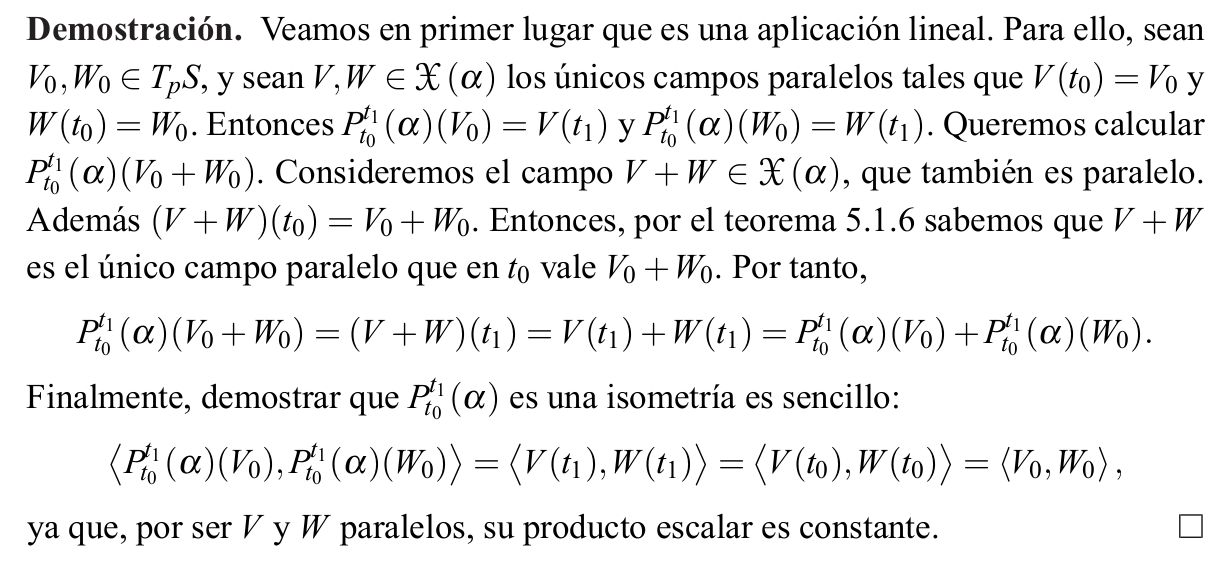
\includegraphics[width=\textwidth]{1.12}





\chapter{Capítulo 2}

\begin{center}
\textbf{Proposición 2.2, la ecuación diferencial extrínseca de las geodésicas}
\end{center}
\begin{demonstration}
  Tenemos la descomposición, por la fórmula extrínseca del campo paralelo,
  $$ \alpha '' (t) = \dfrac{D \alpha '}{dt}(t) +  <\alpha ''(t), N(t)>N(t) \footnote{La manera de obtener esto es considerar $\alpha '$ en lugar de $V$.}$$
  Además, como $\left\langle\alpha^{\prime}(t), N(t)\right\rangle=0$, se tiene $\left\langle\alpha^{\prime \prime}(t), N(t)\right\rangle=-\left\langle\alpha^{\prime}(t), N^{\prime}(t)\right\rangle$. Luego
$$
\frac{D \alpha}{d t}(t)=\alpha^{\prime \prime}(t)+\left\langle\alpha'(t), N^{\prime}(t)\right\rangle N(t) .
$$
  Por lo tanto,
  $$ \alpha \text{ geodésica} \iff \alpha ''(t) + <\alpha '(t), N'(t)>N(t) = \mathbf{0} $$
\end{demonstration}

\begin{center}
\textbf{Proposición 2.6, ecuación diferencial intrínseca de las geodésicas}
\end{center}

\begin{demonstration}
  Utilizando la fórmula que vimos en la primera proposición del tema,
  $$
  V^{\prime}=\left(a^{\prime}+a u^{\prime} \Gamma_{11}^{1}+a v^{\prime} \Gamma_{12}^{1}+b u^{\prime} \Gamma_{12}^{1}+b v^{\prime} \Gamma_{22}^{1}\right) X_{u} + \left(b^{\prime}+a u^{\prime} \Gamma_{11}^{2}+a v^{\prime} \Gamma_{12}^{2}+b u^{\prime} \Gamma_{12}^{2}+b v^{\prime} \Gamma_{22}^{2}\right) X_{v}
  $$

  Ahora, si en lugar de utilizar $V'$ utilizamos $\alpha'$, se tiene $a=u'$ y $b=v'$, y por lo tanto

  $$
  \left\{\begin{array}{l}
  u''+ (u^{\prime})^2 \Gamma_{11}^{1}+2u'v' \Gamma_{12}^{1}+(v^{\prime})^2 \Gamma_{22}^{1}=0 \\
  v''+ (u^{\prime})^2 \Gamma_{11}^{2}+2u'v' \Gamma_{12}^{2}+(v^{\prime})^2 \Gamma_{22}^{2}=0
  \end{array}\right.
  $$
\end{demonstration}
\begin{center}
\textbf{Teorema 2.7, existencia y unicidad de geodésicas}
\end{center}
\textit{En palabras del sensei Alías, 'Hay mejores cosas que preguntar en un examen a parte de este resultado'. Igualmente, os dejo su demostración:}

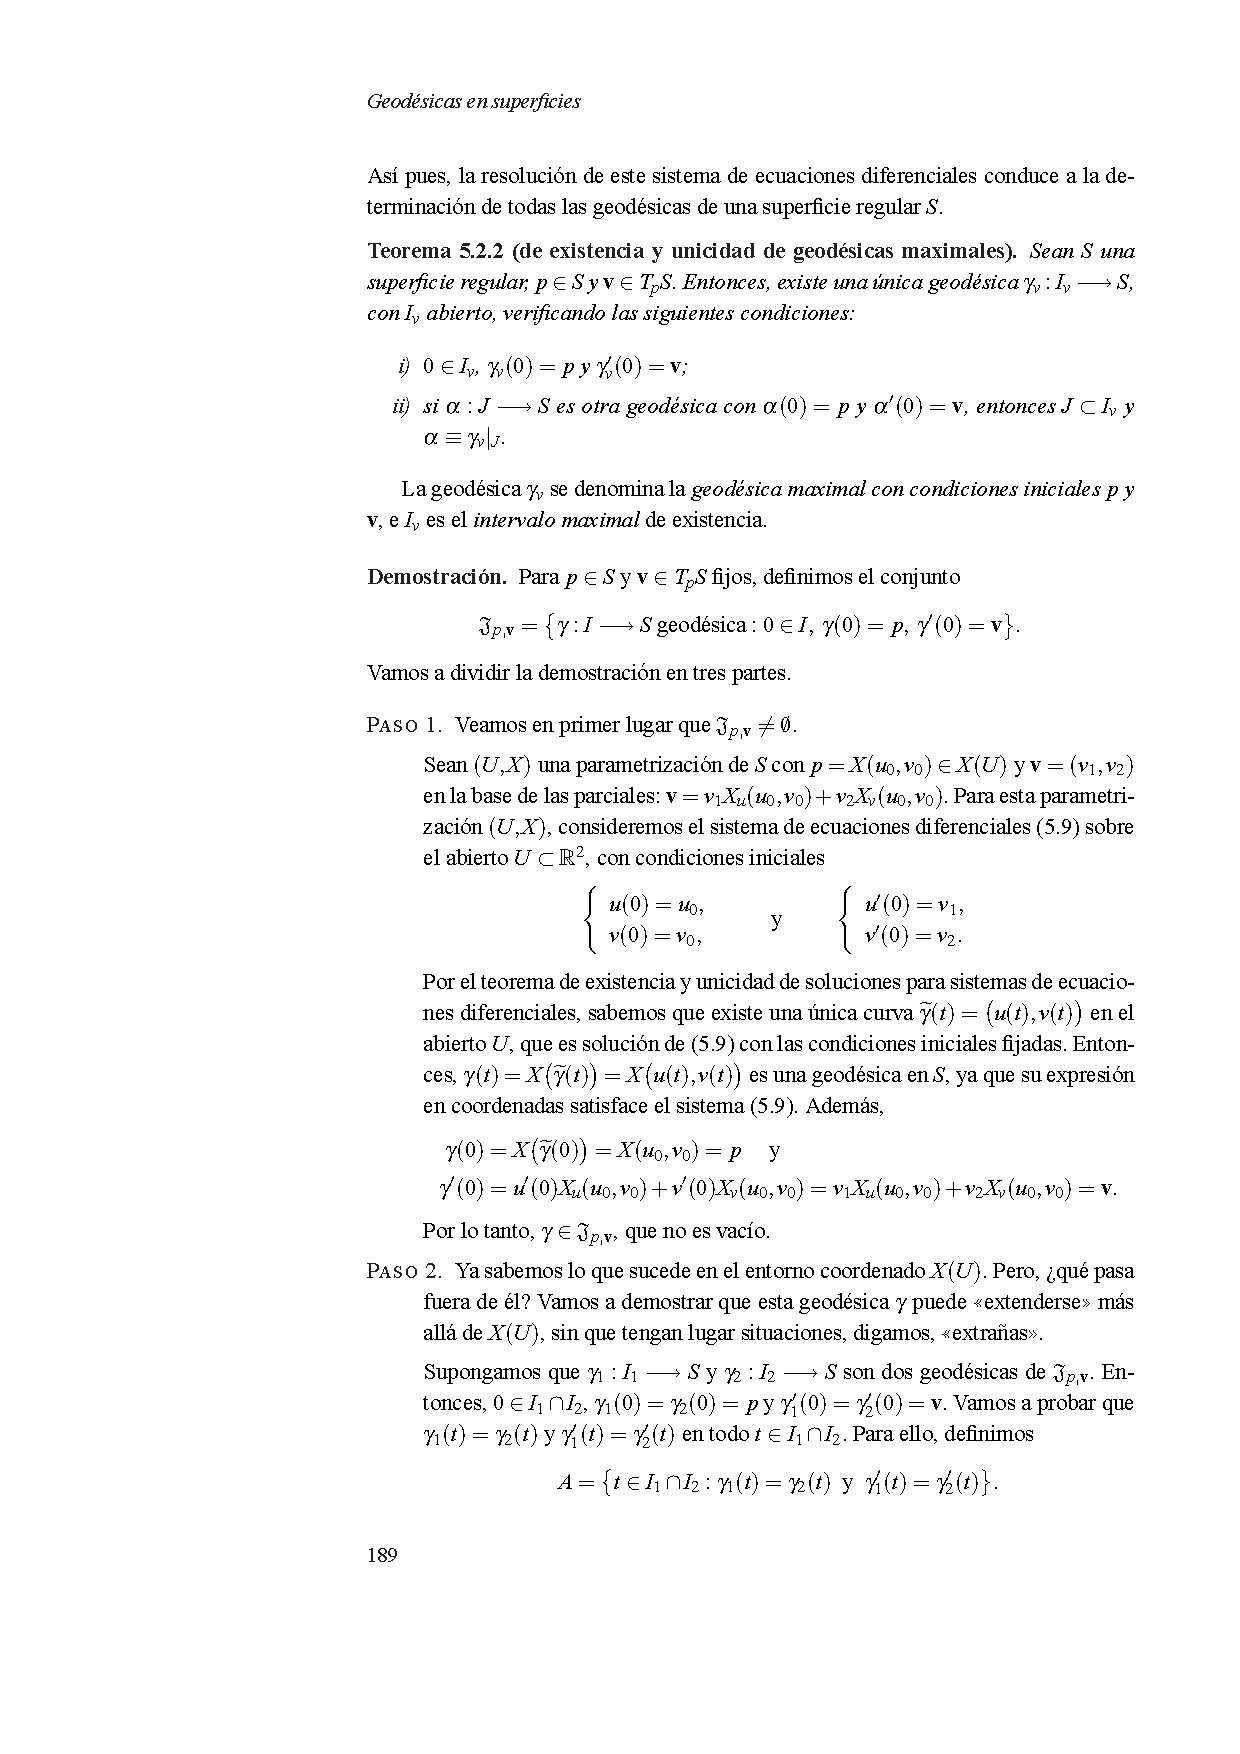
\includepdf[pages=-]{PDFs/2.7.pdf}

\begin{center}
\textbf{Proposición 2.10}
\end{center}
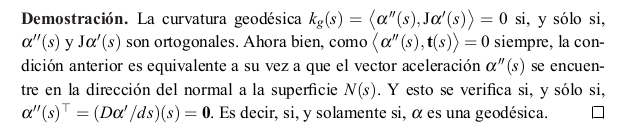
\includegraphics[width=\textwidth]{2.10}

\begin{center}
\textbf{Lema 2.11}
\end{center}
\begin{demonstration}
  Sea $ \beta  $ una reparametrización de $ \alpha  $ que cumpla

  $$ \left\{ \begin{array}{l}
    \beta (s) = \alpha (t(s))\\
    \alpha (t) = \beta (s(t))
  \end{array} \right. $$

$$ k_g^\alpha (t) = k_g^\beta (s(t)) \hspace{1cm} k_g^\beta (t) = <\beta '', J \beta'> = det(\beta '', N, \beta ') $$
$$ \beta (s) = \alpha (t(s)) \to \beta '(s) = t'(s) \alpha '(t(s)) $$

Como $\beta $ está parametrizado por la longitud de arco, entonces

$$ 1=||\beta '(s)||=t'(s) \cdot ||\alpha '(t(s))|| \hspace{1cm}t'(s) = \dfrac{1}{||\alpha '||} $$

$$ \beta '' = t''(s) \alpha '(t(s))  + (t'(s))^2 \alpha ''(t(s))$$

Por lo tanto, $N(s) = N(\beta (s))= N(\alpha (t(s)))$.
$$ k_g^\beta (s) = (t'(s))^3 \cdot det(\alpha ''(t(s)), N(\alpha (t(s))), \alpha '(t(s))) $$
$$ k_g^\beta (s) = \dfrac{det(\alpha '', N \alpha , \alpha ' )}{||\alpha '||^3}(t(s))  $$
$$ k_g^\alpha (t) = k_g^\beta (s(t)) = \dfrac{det(\alpha '', N , \alpha ' )}{||\alpha '||^3}(t)  $$

No entiendo un carajo pero espero que ustedes lo hagan, un saludo.
\end{demonstration}

\begin{center}
\textbf{2.13}
\end{center}
\begin{demonstration}
  Esta queda por hacer...
\end{demonstration}



\begin{proposition}
  { \color{turquoise} \textbf{Proposición exclusiva de \textit{Apuntes PaChito ™}}}

  Sea $\alpha : I \to S \subseteq \mathbb{R}^{ 3 } $ una parametrización. Son equivalentes:

  \begin{enumerate}
    \item $\alpha$ es pregeodésica
    \item $\exists \beta (u) = \alpha (h(u))$ una reparametrización de $\alpha /\beta $ es geodésica.
    \item La reparametrización parametrizada por el arco de $\alpha $ es geodésica.
  \end{enumerate}
\end{proposition}
\begin{demonstration}
  $$ 1 \implies 2 $$

  Directo por la definición

  $$ 3 \implies 1 $$

  Por la definición directo

  $$ 2 \implies 3 $$

  ¿Te imaginas que es directo por la definición? Pues no. Mala suerte.

  Tomamos una reparametrización de $I$:

  $$ I \to^\alpha S $$
  $$ J \to^{h(u)} I $$
  $$ J \to^{\beta (u) = \alpha (h(u)) \text{ que es geodésica}} S $$

  Esto es un triangulito si lo dibujáis... Estaría bien que yo también lo hiciera pero soy un \textit{vago}.

  $$ ||\beta '(u)||= c = h'(u) \cdot ||\alpha '(h(u))|| $$

  Si $c=1 \to \beta (u)$ es la reparametrizavión por arco de $\alpha $

  Si $c \ne 1 \to $ Tomo $\underbrace{ \gamma (s) = \beta(\frac{u}{c}) }_{ GEODESICA } = \alpha (h(\frac{u}{c}))$
  $$ \gamma '(s) = \dfrac{1}{c} \cdot  \beta'\left(\frac{s}{c}\right) $$
\end{demonstration}











\chapter{Capítulo 3}

\begin{center}
\textbf{Lema 3.2, Lema de homogeneidad de las geodésicas}
\end{center}
  Lo más importante del lema son las fórmulas que aparecen centradas en su enunciado.

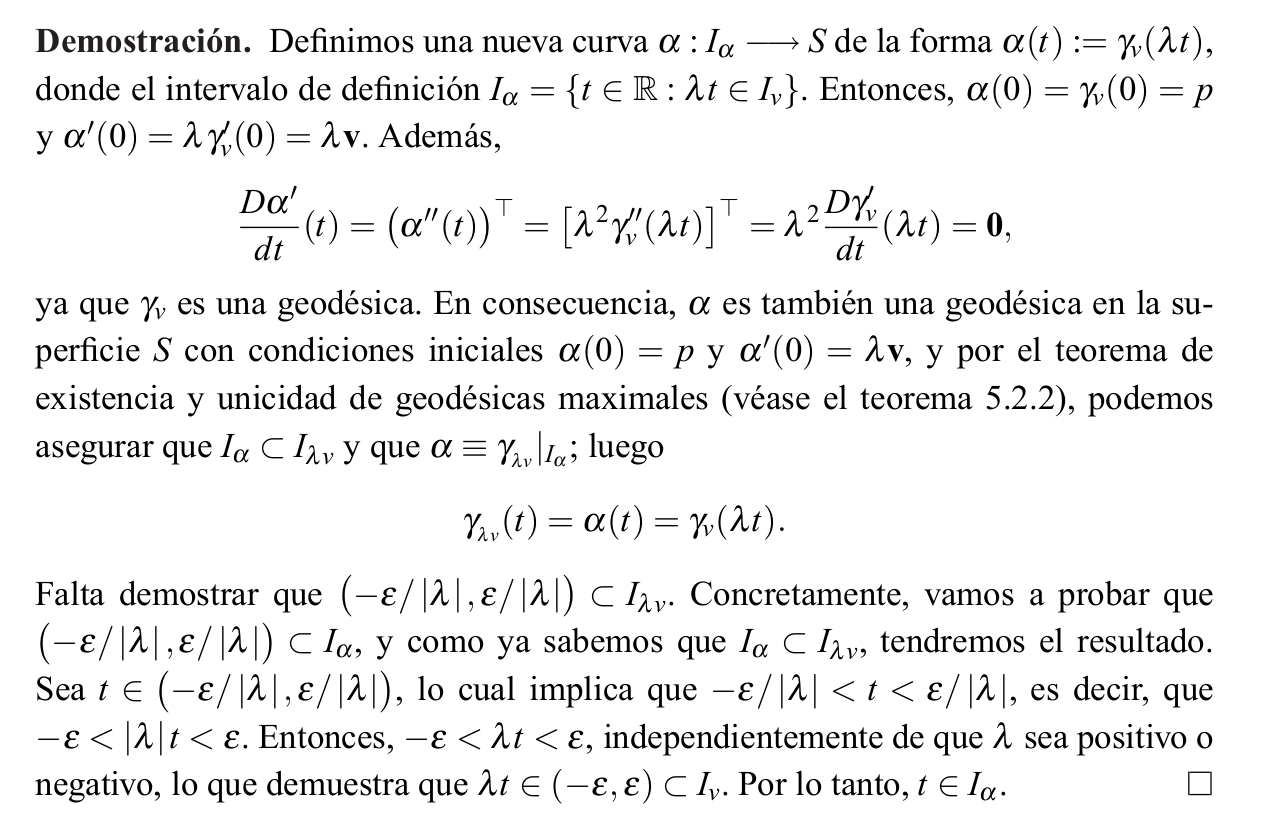
\includegraphics[width=\textwidth]{3.2}
\newpage
\begin{center}
\textbf{Teorema 3.3, Propiedades de la aplicación exponencial}
\end{center}

Primero tenemos que demostrar esta propiedad
$$ p \in S, \ v \in T_pS \implies  iv \in \mathcal{D} _p, \ \forall t \in I_v \supset (- \varepsilon , \varepsilon ) $$
\begin{demonstration}
  $$ \left\{ \begin{array}{l}
    t=0 \to OK\\
    t \ne 0, \hspace{1cm} tv \in \mathcal{D}_p \iff 1 \in I_{tv} = \dfrac{1}{t} \cdot I_v\ si\ 1=\dfrac{1}{t}t
  \end{array} \right. $$
  $$ exp_p(tv) = \gamma _{tv}(1) = \gamma _v (t) , \ \forall t \in I_v $$
\end{demonstration}
Fin de la demostración inciso, comenzamos a demostrar el teorema.
\begin{demonstration}
  $$ I $$
  Que sea estrellado nos dice que el segmento que une cualquier punto con el origen no se sale del conjunto. En otras palabras,
  $$ \forall \underbrace{ v \in \mathcal{D}_p }_{ 1 \in I_v \implies [0,1] \subset I \ \forall t \in [0,1] }, \ [0,v] = \{ tv, \ 0 \leq t \leq 1 \} \subset \mathcal{D}_p $$

  Del inciso se deduce que $t \in I_v \implies tv \in \mathcal{D}_p$. Notamos lo siguiente:
  $$ \forall v \in T_pS, \ \exists (- \varepsilon , \varepsilon ) \subset I_v $$
  Y justo debajo ha escrito
  $$ \exists \varepsilon > 0 \ : \ \forall |t| < \varepsilon , \ tv \in \mathcal{D}_p $$
  $$ II $$
  Este dice el sensei Alías que nos lo creamos y yo \textbf{me lo creo.}
  $$ III $$
  $$ \exists \underbrace{ U }_{ \text{entorno de }0 }\footnote{Para el sensei Alías, decir entorno implica que es abierto} \in \mathcal{D}_p \ : \ exp_{p|\mathcal{U}} \ : \  \underbrace{ \mathcal{U} }_{ \subset T_pS } \to \underbrace{ V }_{ \subset S } \text{ es difeomorfismo}$$

  Para comprobar si es un difeomorfismo, tenemos que ver que la diferencial es un isomorfismo lineal. Vamos a ver si esto es así:

  $$ \forall v \in \mathcal{D}_p \to d(exp_p)_v \ : \ \underbrace{ T_v(\mathcal{D}_p) }_{ T_v(T_pS) } \to T_{exp_p(v)}S $$

  $$ \forall w  \in T_pS \hspace{1cm} \alpha (t) = v + tw $$
  $$ \alpha \ : \ I \to \mathcal{D}_p \subset T_pS $$
  $$ \alpha (0) = v \hspace{1cm} \alpha '(0) = w \hspace{1cm} \to \hspace{1cm}w \in T_v(T_pS)$$

  Vamos al caso particular $v=0$.
  $$ d(exp_p)_0 \ : \ T_0(TpS) = T_pS \to T_{exp_p(v)}S = T_pS$$
  $$ \forall w \in T_pS = T_0(T_pS) $$
  $$ d(exp_p)_v(w) = \dfrac{d}{dt}_{t=0} exp_p(\alpha (t)) $$

  Tenemos que encontrar una curva que cumpla
  $$ \forall \alpha (t) \ : \ (- \varepsilon , \varepsilon ) \to T_pS $$
  $$ \left. \begin{array}{l}
    \alpha (0) = 0\\
    \alpha '(0) = w
  \end{array} \right\} \alpha (t) = t w $$

  $$ exp_p(\alpha (t)) = exp_p(tw) = \gamma _{tw}(1) = \gamma _w(t) $$
  $$ d(exp_p)_0(w) = \gamma '_w(0) = w \implies d(exp_p)_0 = Id $$
\end{demonstration}


\begin{center}
\textbf{Lema 3.6, El lema de Gauss}
\end{center}

Vamos a demostrar una versión más general de lo que viene en los apuntes. En nuestra versión demostraremos
$$ \forall w \in T_pS \hspace{1cm} <d(exp_p)_v(v), d(exp_p)_v(w)> = <v,w> $$
\begin{demonstration}
  Procedo a copiar lo que ponga el sensei en la pizarra. Para demostrar esta propiedad, debemos hacer una cuenta.

  \textbf{Caso fácil:}

  Supongamos $ w=\lambda v $. Entonces, $d(exp_p)_v(w) = \dfrac{d}{dt}_{t=0
  } exp_p(\alpha (t)) , \  \alpha (t) \ : \ (- \varepsilon , \varepsilon ) \to \mathcal{D}_p$. Tomamos $\alpha (t) = v + tw = v + t \lambda v = (1+ \lambda t) v$

  $$ exp_p(\alpha (t))= exp_p((1+\lambda t)v) = \gamma _v(1+ \lambda t) $$
  $$ \dfrac{d}{dt} \gamma _v((1+ \lambda t)v) = \lambda \gamma '_v (1+ \lambda t)$$
  $$ \implies _{t=0} d(exp_p)_v(w)= \lambda \gamma '_v(1) $$

  Ahora, vamos a utilizar que el módulo es constante.

  $$ <d(exp_p)_v(v), d(exp_p)_v(w)> = <\gamma '_v(1), \lambda \gamma '_v(1)> = \lambda ||\gamma '_v(1)||^2 = \lambda ||\gamma '_v(0)||= \lambda ||v||^2 =$$
  $$ =<v,\lambda v>= <v,w>  $$

  \textbf{Caso chungo:}

  Supongamos ahora que $v$ y $w$ son linealmente independientes, que es una condición más general a que sean ortogonales. Este tiene un poco más de miga.

  Consideramos $\phi(s,t) \ : \ \mathbb{R} \times \mathbb{R} \to T_pS$ tal que
  $$ \phi(s,t) = s(v+tw) = s \alpha (t) $$

  En este caso,
  $$ \phi(0,t) = 0 \hspace{0.2cm} \forall t \hspace{1cm} \phi(1,t) = \alpha (t) \hspace{0.2cm}\forall t \footnote{Luis está haciendo un dibujo bastante ilustrativo en la pizarra (hoy es 17 de Febrero, por si os queréis ver la clase). El caso es que el hijo de puta de Paco aún no se ha puesto a tomar apuntes conmigo (es cuestión de tiempo, siempre se mete el jodido) y no me da tiempo a copiar lo que dice y el dibujo, así que... Lector, good luck.}$$

  Si $ \alpha  \in \mathcal{D}_p$ entonces
  $$ \phi(s,t) \in \mathcal{D}_p , \ \forall s \in [0,1] $$
  $$ \phi(s,t) \in \mathcal{D}_p , \ \forall s \in (- \varepsilon ', 1+ \varepsilon ') $$
  $$ \alpha (0) \in \mathcal{D}_p \to \exists \varepsilon >0 | \alpha (t) \in \mathcal{D}_p, \ \forall |t| < \varepsilon  $$

  Por compacidad, $\exists \varepsilon >0 \ | \ \phi(s,t) \in \mathcal{D}_p , \ \forall (s,t) \in (- \varepsilon , 1+\varepsilon ) \times (-\varepsilon , \varepsilon )$. Ahora, considero la siguiente aplicación $$\psi(s,t) = exp_p(\phi(s,t)) = exp_p(s\alpha (t))$$
  $$ \alpha (t) = v + tw $$
  $$ \psi \ : \ (-\varepsilon , 1 + \varepsilon ) \times (-\varepsilon , \varepsilon ) \to ^\phi \mathcal{D}_p \to ^{exp_p} S, \text{ que es bien definida y }C^\infty  $$
  $$ exp_p(s\alpha (t)) = \gamma _ {\alpha(t)}(s) $$

  La derivada fácil de $\psi$ es con respecto de $s$ y por ella vamos a comenzar.

  $$ \dfrac{\partial \psi}{\partial s}(s,t) = \dfrac{d }{ds}_{t=cte}(\gamma _ {\alpha (t)} (s)) = \gamma '_{\alpha (t)}(s) \hspace{1cm} \dfrac{\partial ^2 p}{\partial s^2}  (s,t) = \gamma ''{\alpha (t)}(s) \text{ normal}$$
  $$ \dfrac{\partial \psi}{\partial s}(s,t) = \dfrac{\partial }{\partial s}(exp_p(s \alpha (t))) = d(exp_p)_{s(\alpha (t))}(\alpha (t))  $$
  $$ \dfrac{\partial \psi}{\partial s}(s,0) = d(exp_p)_{s,v}(v) = \left\{ \begin{array}{l}
    d(exp_p)_0(v) = v, \ s=0\\
    d(exp_p)_v(v) , \ s=1\\
  \end{array} \right.  $$

  $$ \dfrac{\partial \psi}{\partial s}(1,0) = d(exp_p)_v(v)  $$


  Bueno si este ha sido el caso fácil agárrate de los pelos que vamos a derivar con respecto de $t$.

  $$ s=0 \to \psi(0,t) = exp_p(0) = p $$
  $$ s=1 \to \psi(1,t) = exp_p(\alpha (t)) \to \dfrac{\partial p}{\partial t}(1,t) = d(exp_p)_ {\alpha(t)} (\alpha (t)) = d(exp_p)_{\alpha (t)}(w) $$
  $$ \dfrac{\partial \psi}{\partial t}(1,0) = d(exp_p)_v(w)  $$
  $$ <\dfrac{\partial \psi}{\partial s}(1,0), \dfrac{\partial \psi}{\partial t}(1,0)>= ?? $$
  $$ f(s) = < \dfrac{\partial p}{\partial s}(s,0), \dfrac{\partial \psi}{\partial t}(s,0)> , \ \forall s \in [0,1] $$

  Mi objetivo es calcular $f(1)$.
  $$ f'(s) = \underbrace{ <\dfrac{\partial ^2 \psi}{\partial s^2}(s,0) , \ \dfrac{\partial \psi}{\partial t}(s,0)> }_{ A } + \underbrace{ <\dfrac{\partial \psi}{\partial s}(s,0), \dfrac{\partial ^2\psi}{\partial t \partial s}(s,0) > }_{ B }   $$

  $$ \dfrac{\partial ^2 \psi}{\partial s^2}(s,t) = \gamma ''_{\alpha (t)}(s)  $$
  $$ \dfrac{\partial ^2 \psi}{\partial s^2}(s,0) = \gamma ''_v \text{ normal a }S \text{ en } \gamma _v(s) $$
  $$ \dfrac{\partial \psi}{\partial t}(s,0) = \dfrac{\partial }{\partial t}\left( \psi(s,t) \right) = \beta '_s(0) \in TS=T   $$

  A tomar por culo, os lo copio del libro:
\end{demonstration}

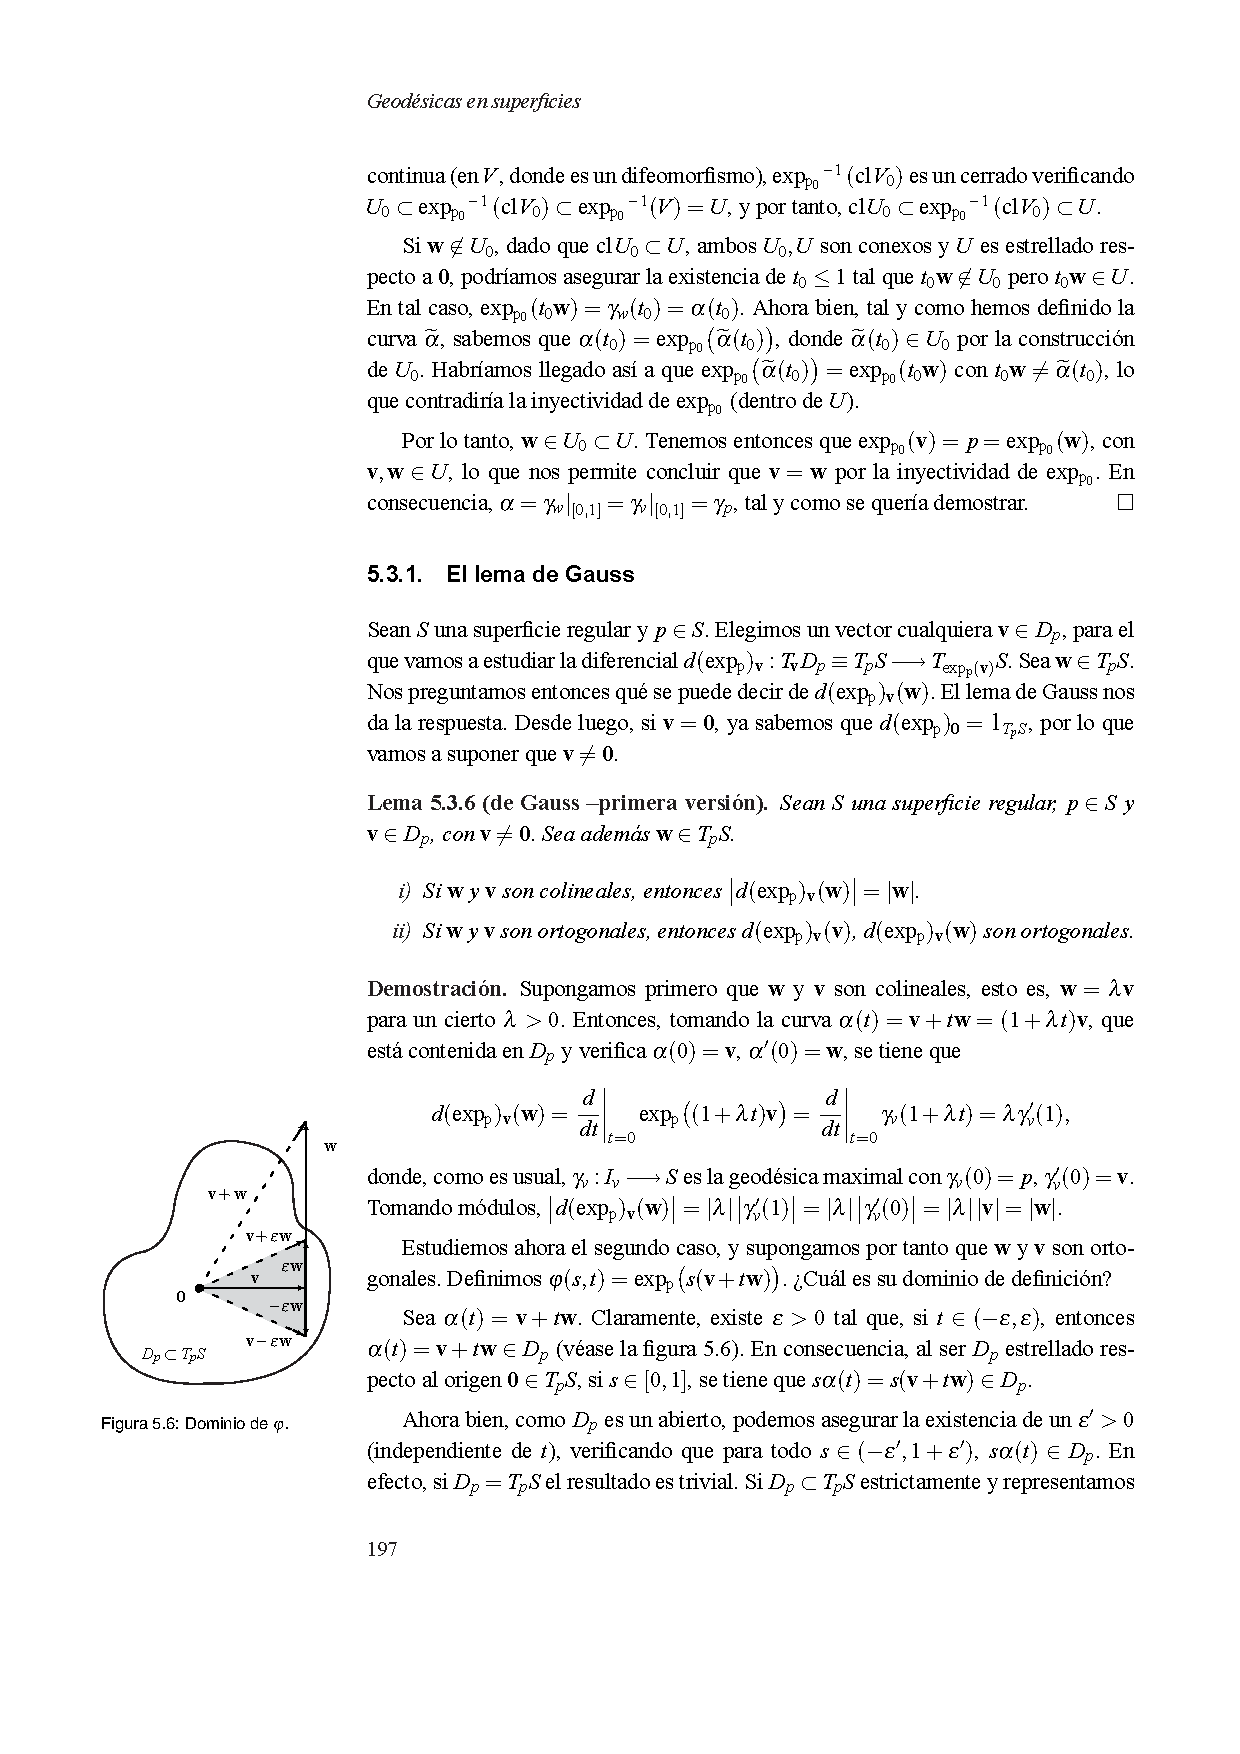
\includepdf[pages=-]{PDFs/3.6.pdf}

\hspace*{-4cm}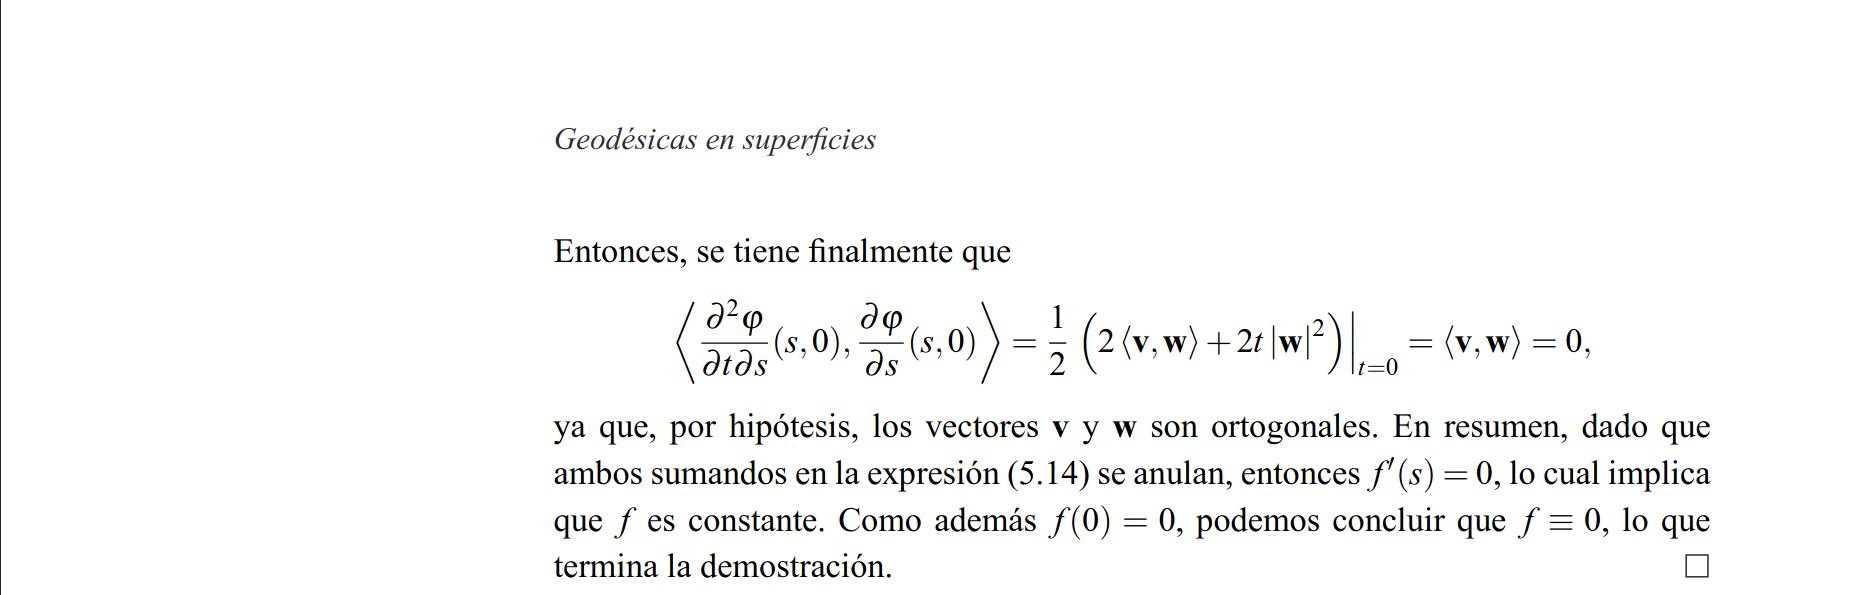
\includegraphics[width=\paperwidth]{3.6}


\begin{center}
\textbf{Teorema 3.8, Propiedad minimizante de las geodésicas}
\end{center}

Es bastante difícil poner con palabras cuán horrenda, larga y desagradable es esta demostración. Por esto, he decidido meter aquí su equivalente en el libro tal cual y sin ningún tipo de respeto. Por si os surgen dudas y queréis consultar la fuente, es el teorema 5.3.9 del curso de Hernández Pastor. Comienza en la siguiente página.

Os animo a hacer un dibujo libre en lo que queda de página y enviármelo por twitter al user @chitobelm.

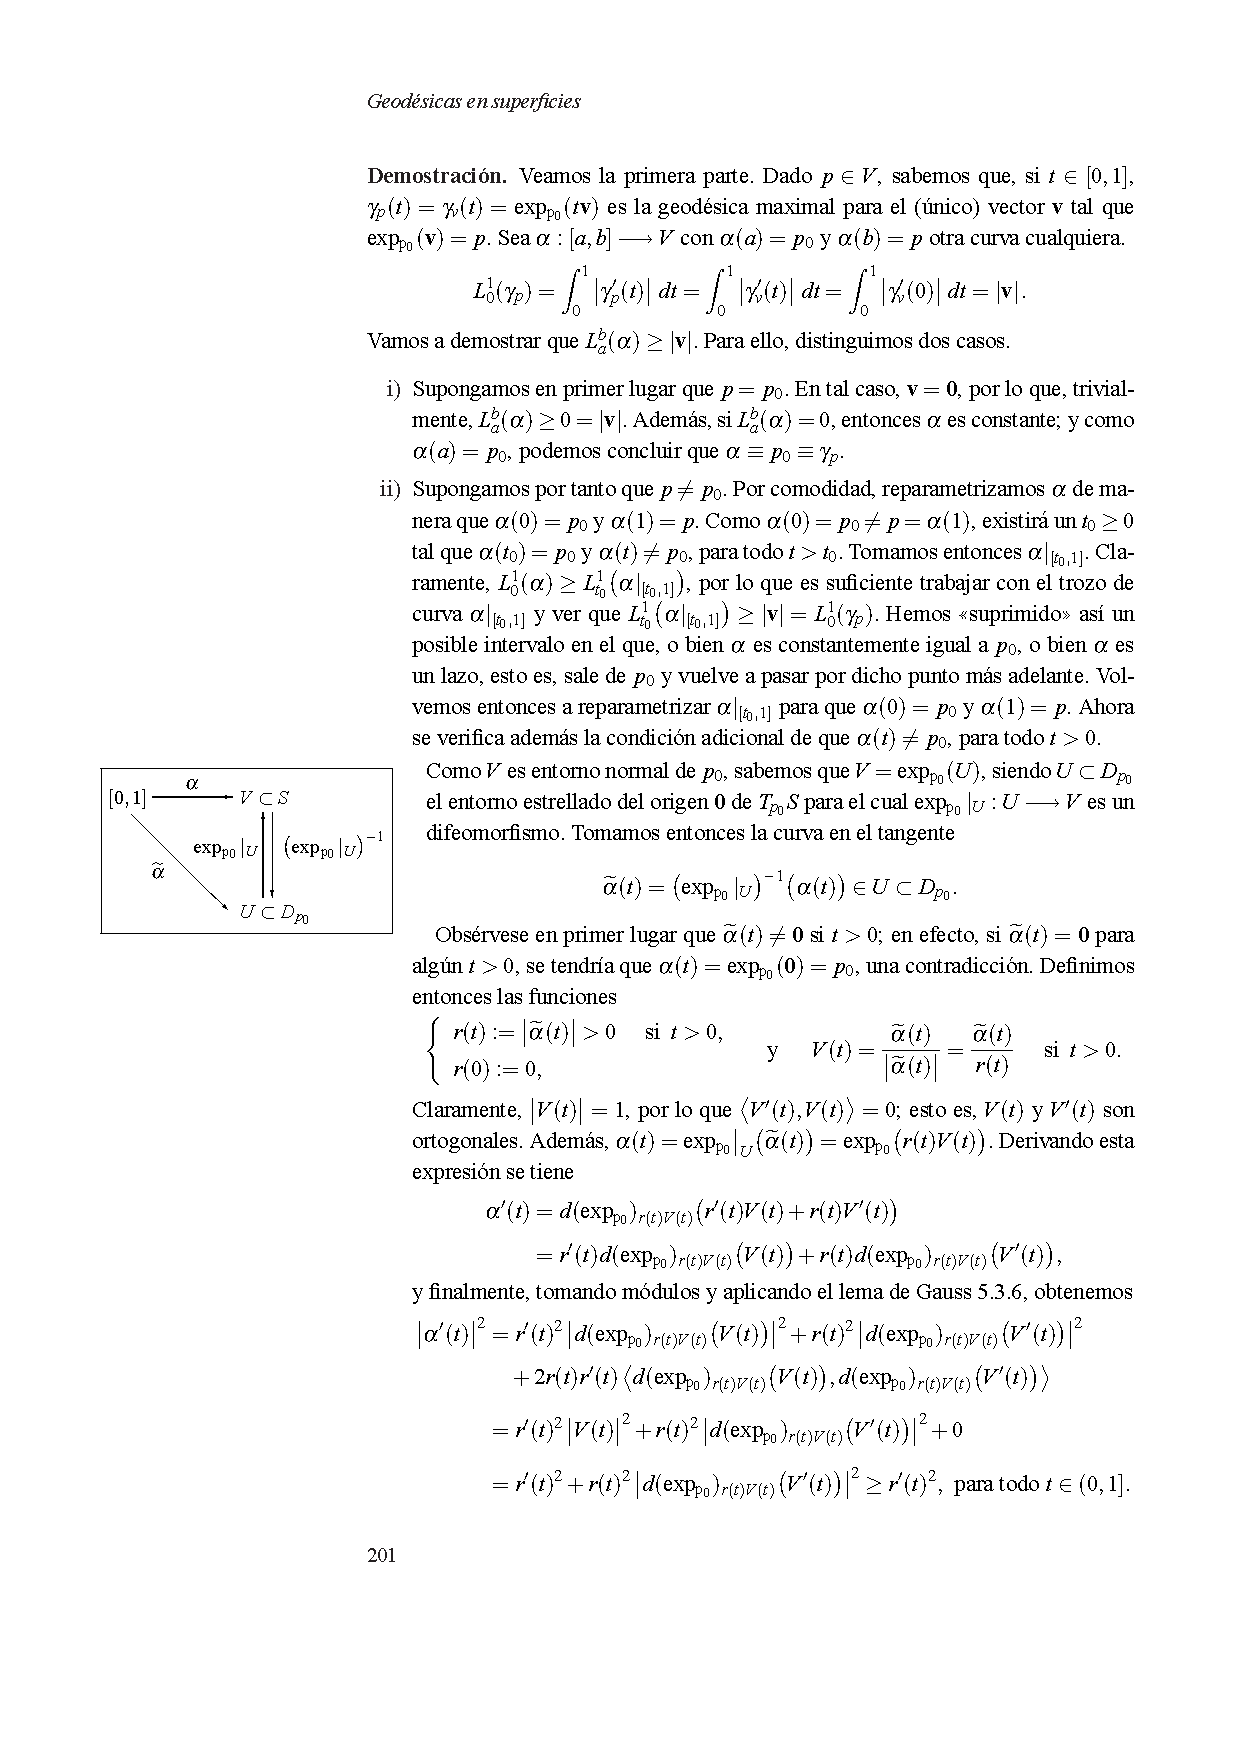
\includepdf[pages=-]{PDFs/propiedadMinimizante.pdf}


\begin{center}
\textbf{Teorema 3.9}
\end{center}


\begin{center}
\textit{Inciso, más adelante se hace referencia a 4.2, se refiere a esto}
\end{center}
\begin{center}
  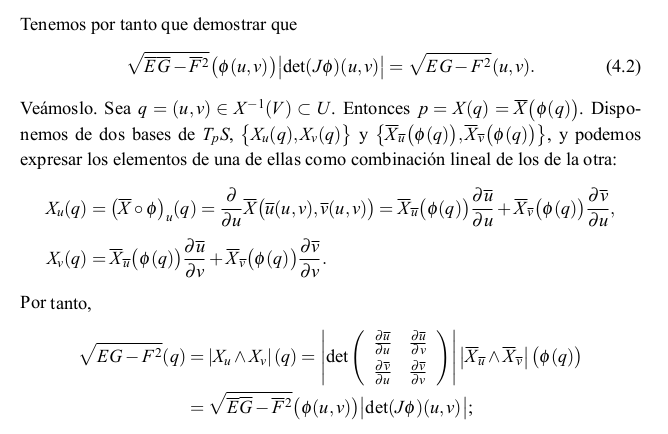
\includegraphics[scale=0.6]{3.9 inciso}
\end{center}
\hspace*{-4cm}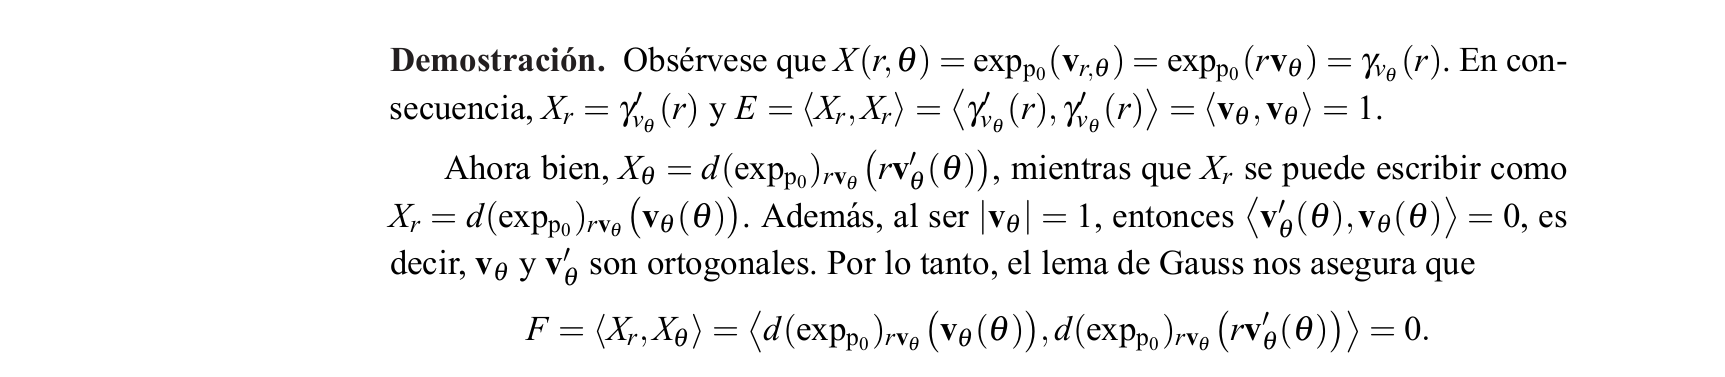
\includegraphics[width=\paperwidth]{3.9 1}
\newpage
\hspace*{-4cm}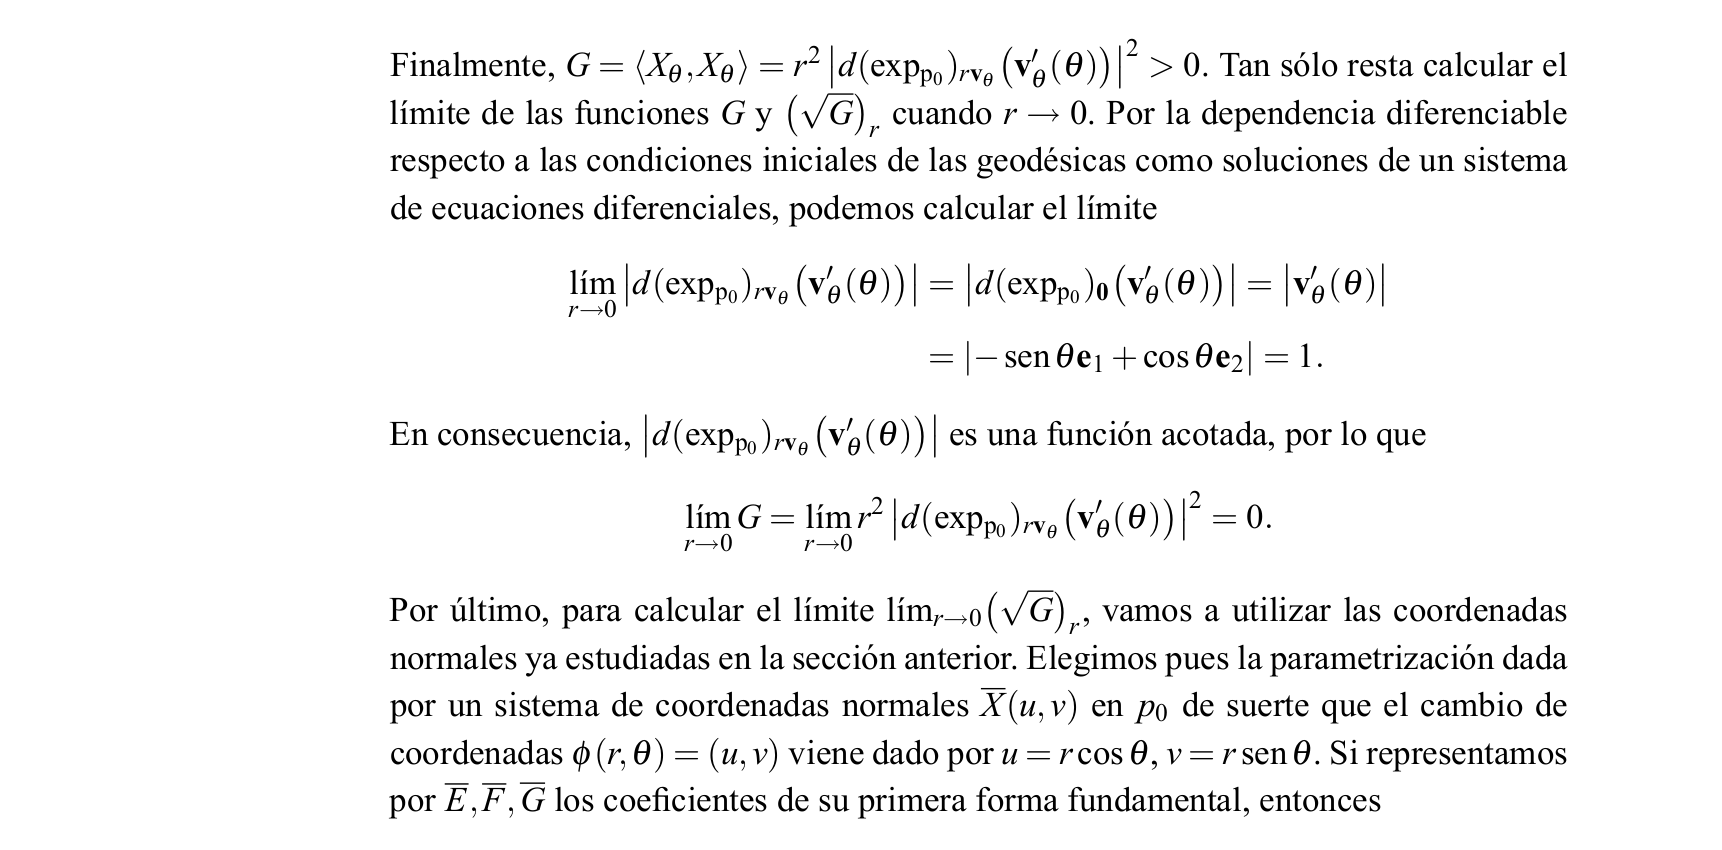
\includegraphics[width=\paperwidth]{3.9 2}
\hspace*{-4cm}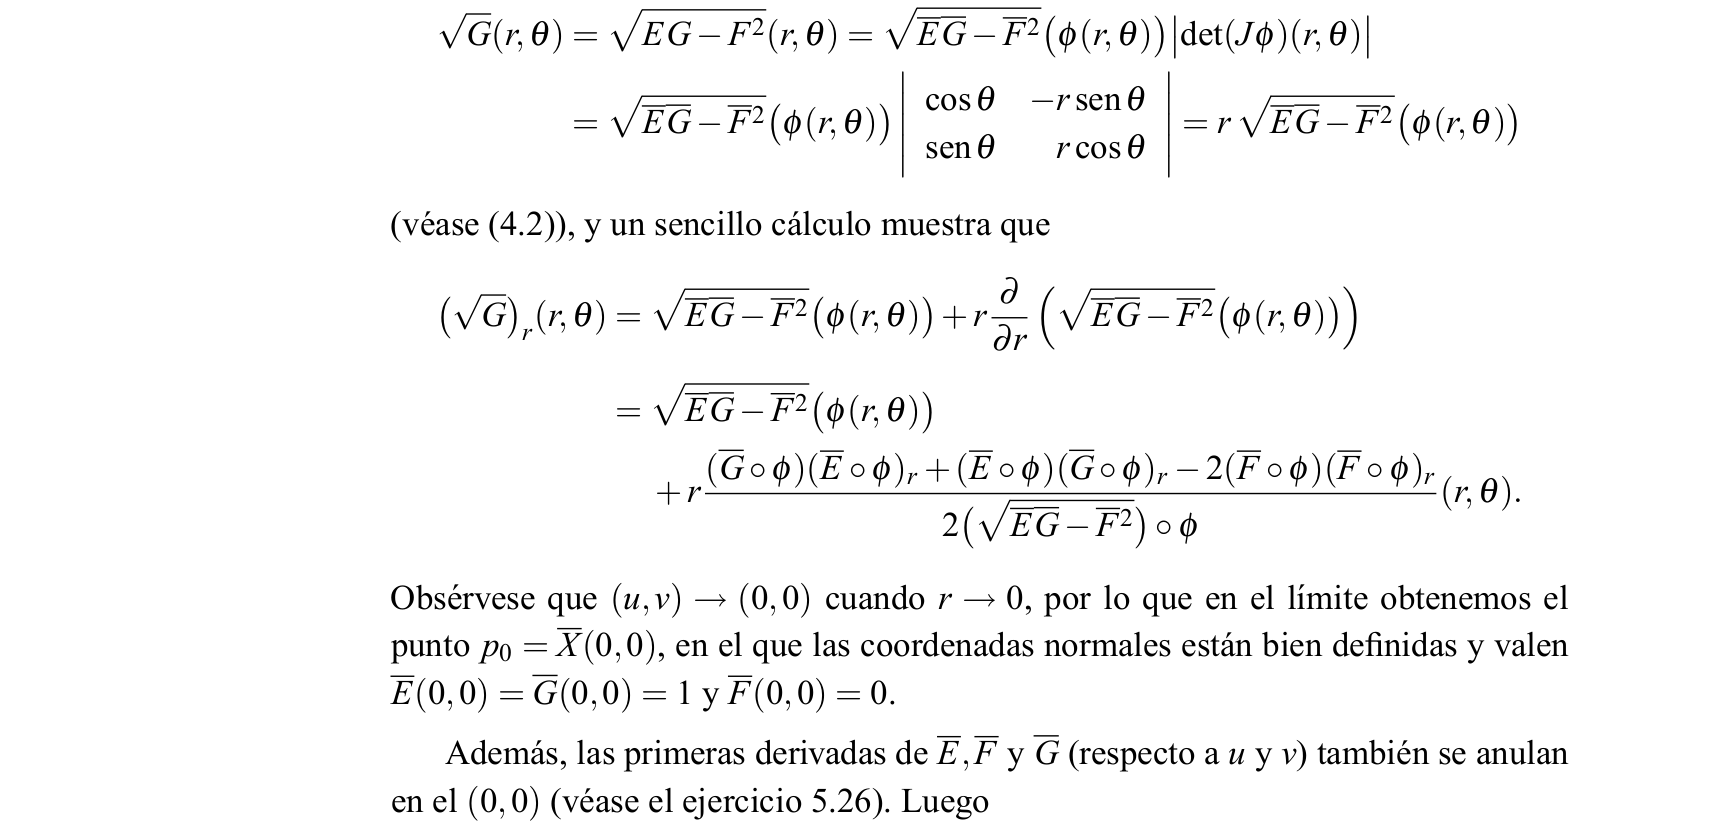
\includegraphics[width=\paperwidth]{3.9 3}
\hspace*{-4cm}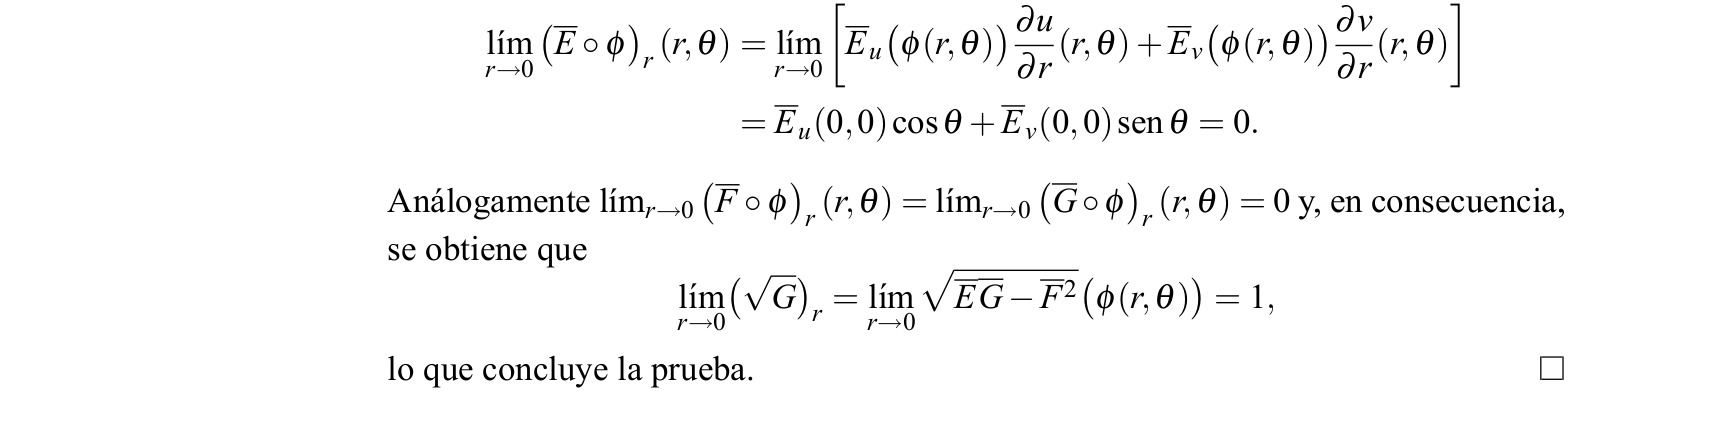
\includegraphics[width=\paperwidth]{3.9 4}

\begin{center}
\textbf{Teorema de Minding}
\end{center}
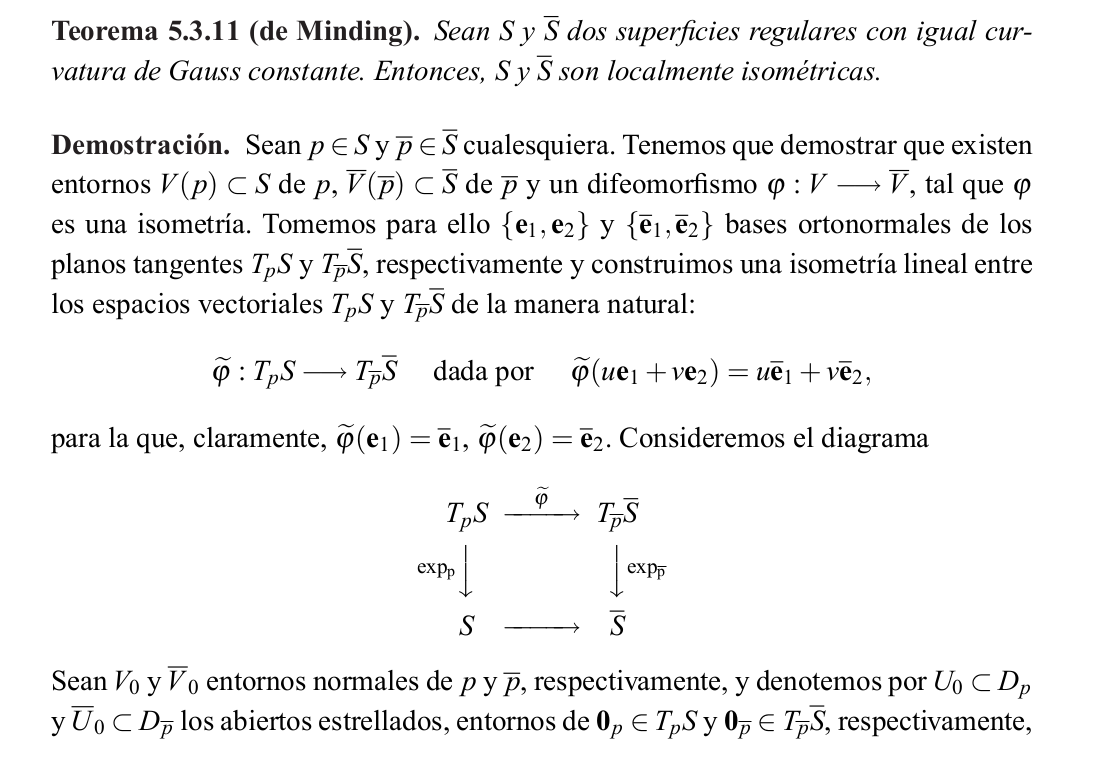
\includegraphics[width=\textwidth]{minding}
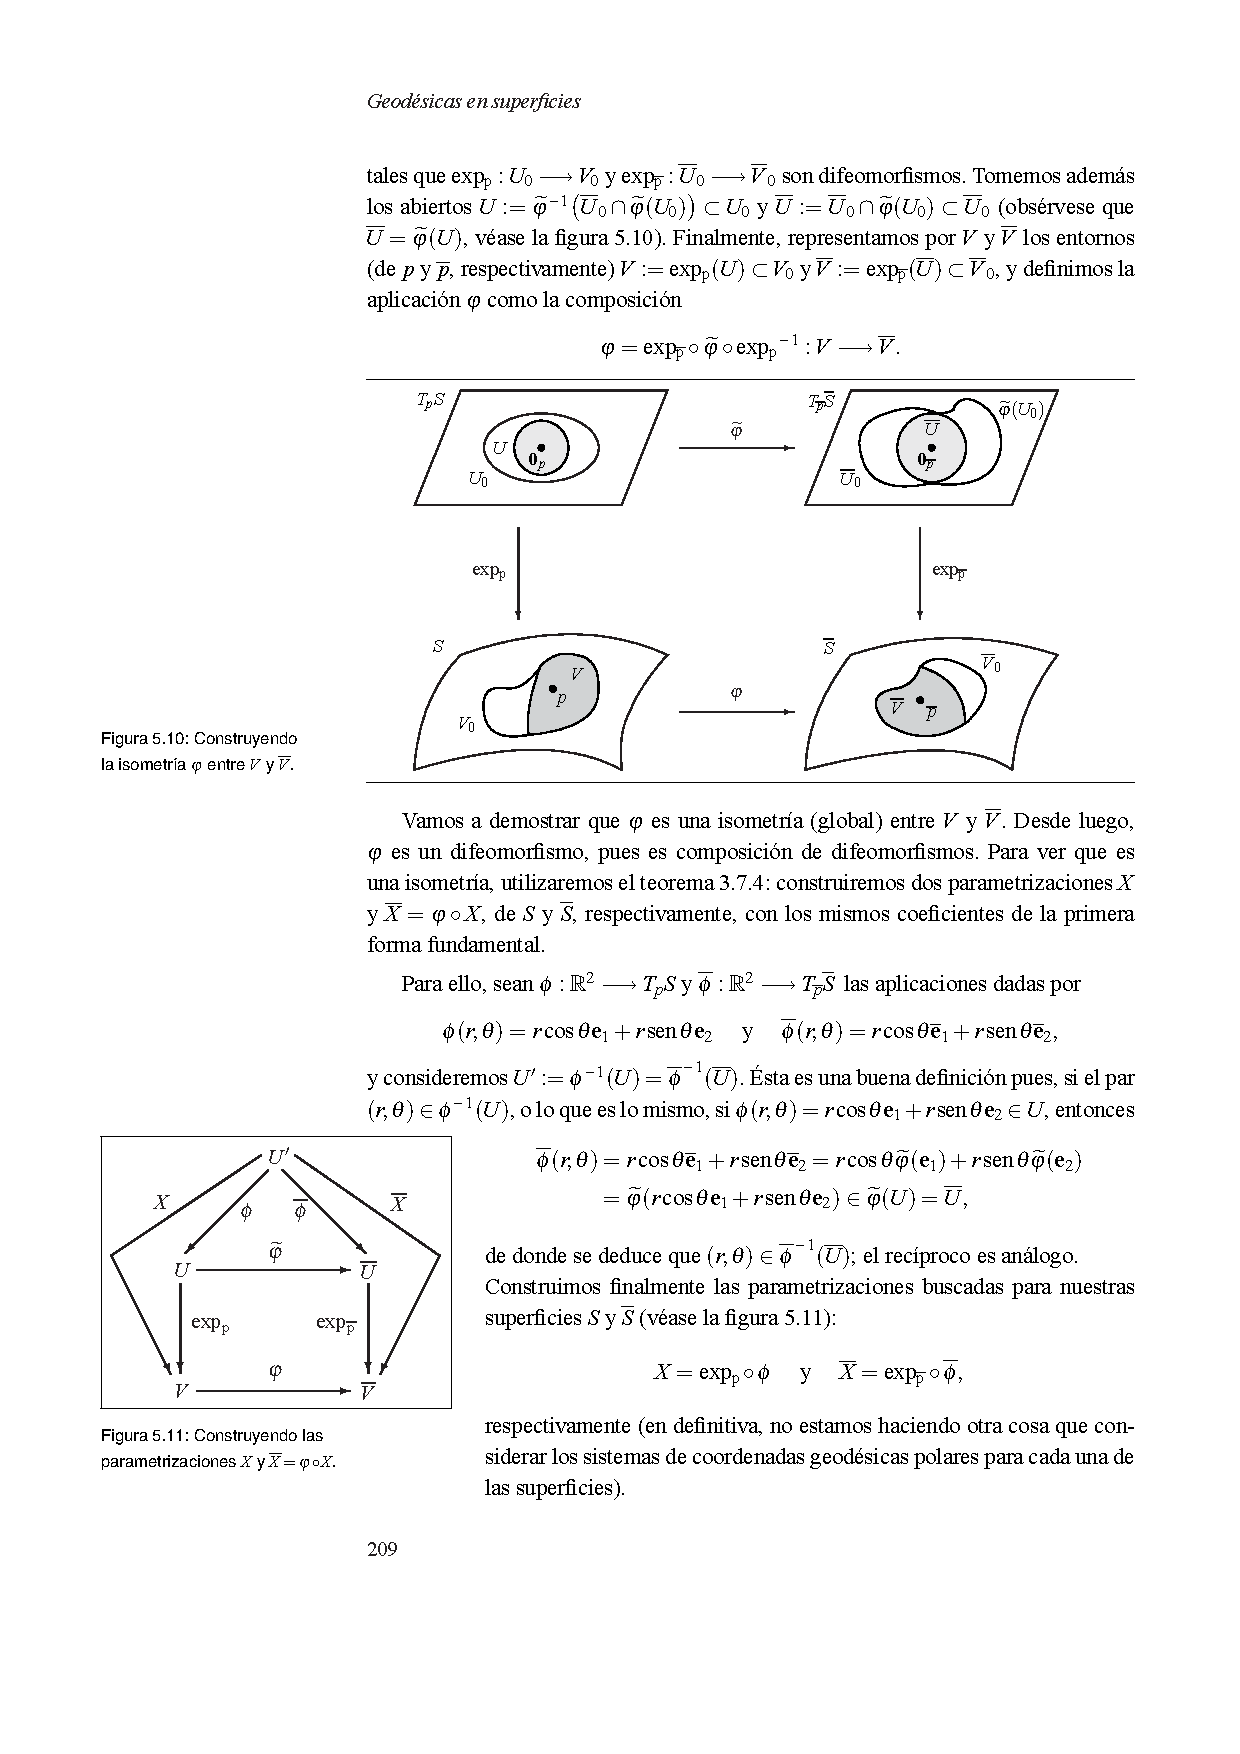
\includepdf[pages=-]{PDFs/minding.pdf}

\part{Parte 2}

\chapter{Capítulo 4}


\begin{center}
\textbf{Lema 4.3}
\end{center}

\begin{center}
\textbf{Enunciado I}
\end{center}

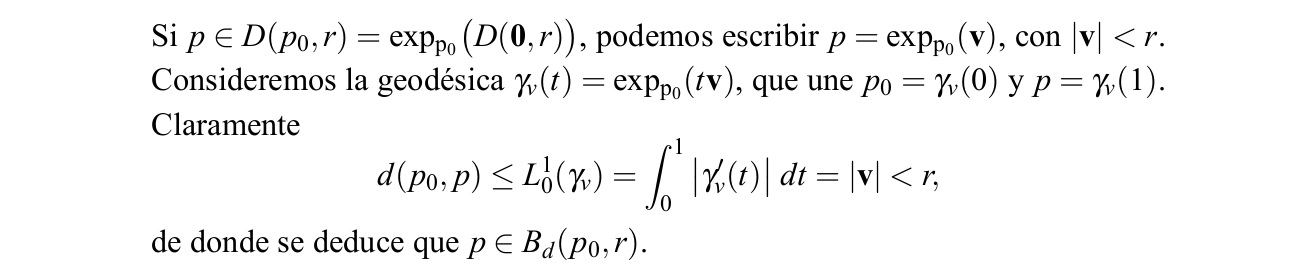
\includegraphics[width=\textwidth]{4.3i}


\begin{center}
\textbf{Enunciado II}
\end{center}

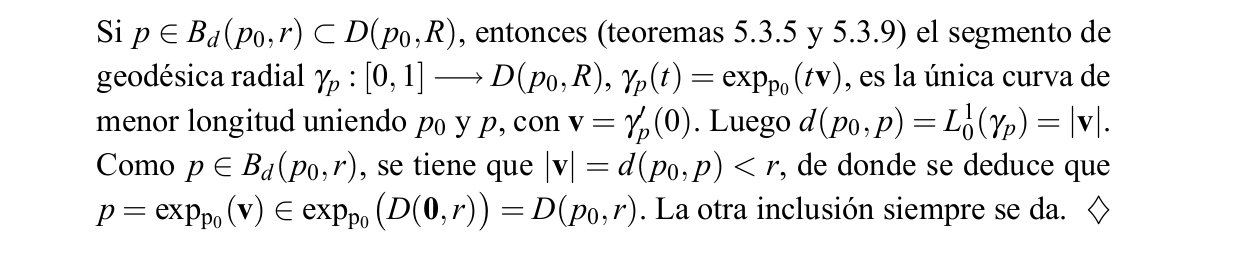
\includegraphics[width=\textwidth]{4.3ii}


\textit{Inciso: los teoremas que se mencionan se refieren a la existencia y unicidad de geodésicas radiales.}
\newpage
\begin{center}
\textbf{Corolario 4.4}
\end{center}

\textit{En la demostración, }$\tau_d$\textit{ es la topología inducida por la distancia intrínseca. Yo, personalmente, supongo que }$\tau_u$\textit{ es la topología de la superficie S, pero qué voy a saber yo, si sólo soy un Pokémon de tipo Normal...}

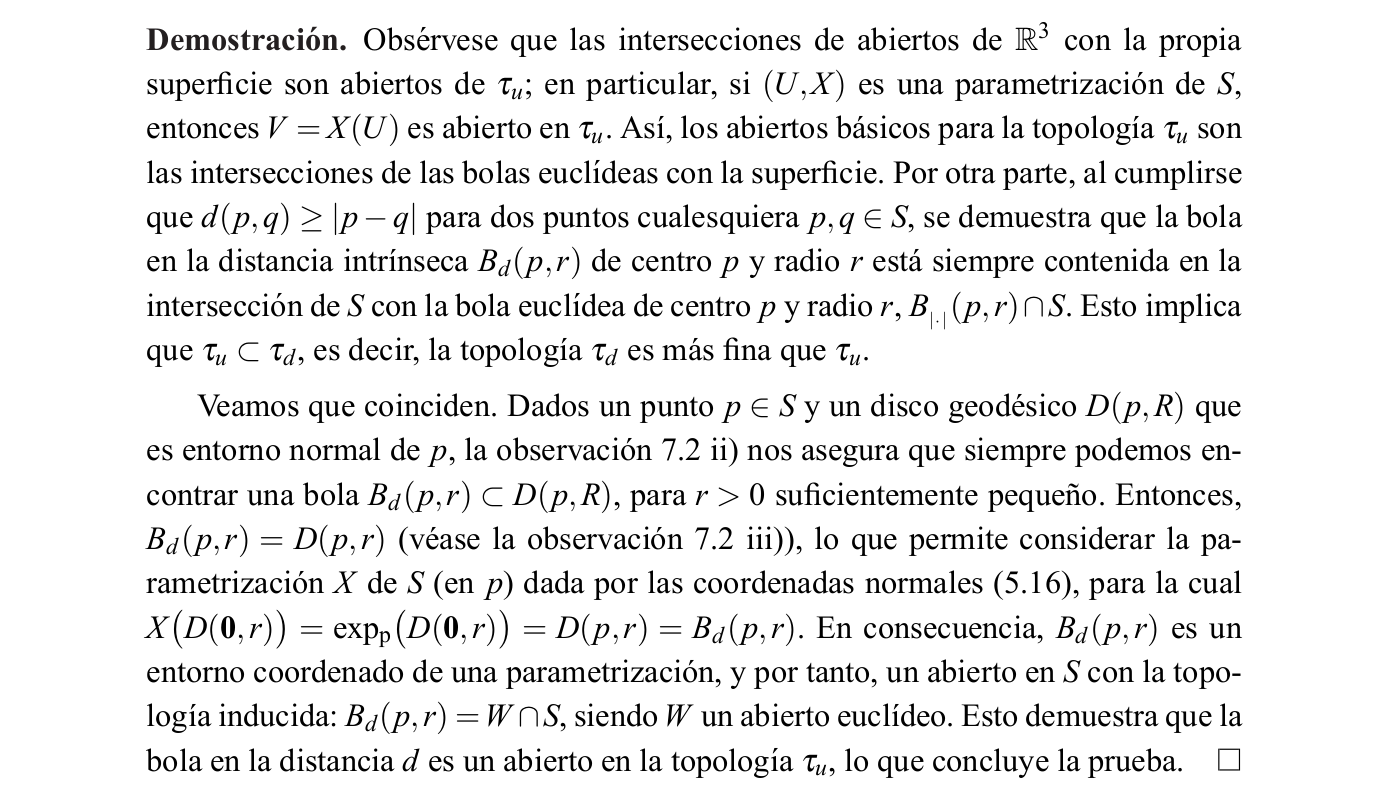
\includegraphics[width=1.1\textwidth]{4.4}


\chapter{Capítulo 5}

\textit{La demostración que está apuntada aquí abajo está tomada por mi compa el Paco en clase. Como no está extraída del libro, ninguno de los autores se hace responsable de cuán caótica o sinsentido pueda resultar. Como decía mi padre: haber estudiao.}
\begin{center}
\textbf{Propiedad del corolario 5.4}
\end{center}
\begin{demonstration}

  Quiero demostrar que si $ \alpha  \in [a,b] \to  V$ es un segmento de geodésica tal que $\alpha (a) = p_0$ y $\alpha (b) = p$, entonces $\alpha $ es una reparametrización de $\gamma _p$.

  Reparametrizamos $\alpha $ para que esté definida entre $0$ y $1$, en primer lugar. Defino $$\beta (t)=\alpha ((1-t)a+tb):[0,1] \to V \hspace{1cm} \left\{\begin{array}{l}
    \beta (0)=p_0\\
    \beta (1)=p
  \end{array}\right.$$

  Sabemos que $\gamma _p(t) = exp_{p_0}(t v_p)$. Definimos $w= \beta '(0) \in T_{p_0}S$. Existe entonces $\gamma _w : I_w \to S$ una geodésica maximal.

  ¿Cómo se relacionan $ \beta  $ y $ \gamma _w $? Hasta ahora, sabemos:
  $$ \left\{\begin{array}{l}
    \gamma _w(0) = p_0 = \beta (0)\\
    \gamma'_w(0) = w = \beta (0)
  \end{array}\right. \implies [0,1] \subset I_w \text{ y además } \beta (t) = \gamma _w (t)\ \forall t \in [0,1]$$

  Tenemos tres sucesos elementales ahora:

  $$ exp_0(v_p)=p \hspace{1cm} exp_{p_0}(w) = \beta (1) = p \hspace{1cm}exp_{p_0|\mathcal{U}}: U \to V \text{ es un difeomorfismo.} $$

  Nos falta demostrar que $w \in \mathcal{U}$. Vamos a probarlo.

  \begin{center}
  \textbf{Prueba de que w está en U}
  \end{center}

  Sé que $\beta (t) \in V, \ \forall t \in [0,1]$. Tenemos $\overline{\beta }(t) = \left( exp_{p_0 | \mathcal{U}} \right)^{-1} (\beta (t)) : [0,1] \to \mathcal{U}$.

  $$ \beta (t) = exp_{p_0}(\overline{\beta }(t)) , \ \forall t \in [0,1] $$

  Mi objetivo es demostrar que $\overline{\beta }(t) = tw, \ \forall t \in [0,1]$. Entonces, podría argumentar que $\overline{\beta }(1) = w \in \mathcal{U}$.

  Llamo $A= \{ t \in [0,1) \ : \  \overline{\beta }(t) = tw  \}$.
    \begin{enumerate}
      \item $0 \in A$, luego $A \ne \emptyset$, $\overline{\beta}'(0) = 0=0 \cdot w$.
      \item $A$ es cerrado, $f(t) = ||\overline{\beta }(t) - tw || , \ f:[0,1] \to \mathbb{R}$, $A= f ^{-1} (0)$.
      \item $A$ es abierto, esto es más complicado.

      Dado $t_0 \in A$, ¿$\exists \varepsilon >0 | (t_0 - \varepsilon , t_0 + \varepsilon ) \subset A$?

      $$ t_0 \in A \implies \overline{\beta }(t_0) = t_0 w \in \mathcal{U} $$
      $$ \exists \varepsilon >0 \ | \ tw \in \mathcal{U} , \ \forall t \in (t_0 \pm \varepsilon )$$
      $$ \beta (t) = exp_{p_0}(tw) = exp_{p_0}(\overline{\beta }(t))\in \mathcal{U} \hspace{0.4cm} \forall t \in (t_0 \pm \varepsilon ) \implies $$
      $$ \implies \overline{\beta }(t) = tw \hspace{0.4cm} \forall t \in (t_0 - \varepsilon , t_0 + \varepsilon )  $$
    \end{enumerate}
\end{demonstration}


\begin{center}
\textbf{Corolario 5.4}
\end{center}

\textbf{TODO: CONSULTAR KARBAJOAPUNTES}

\begin{demonstration}
  Tomo $W$ un entorno convexo de $ p $. Tenemos garantizado que $\exists a<b \ : \ \gamma (a) \in W$. $W$ es también, ahora, un entorno normal de $\gamma (a)$.

  Tomamos una reparametrización $\alpha = \gamma |_{[a,b]}: [0,1] \to W$, que es un segmento de geodésica que une $\gamma (a)$ con $\gamma (b)$.

  Definamos ahora $\gamma _p: [0,1 + \varepsilon) \to W$ segmento de geodésica radial que une $\gamma (a)$ con $\gamma (b)$.
\end{demonstration}


\begin{center}
\textbf{Lema 5.6}
\end{center}
\textit{Este es el lema 7.2.3 del libro de la bibliografía. Su longitud excede lo que considero oportuno para que un ser humano sufra en una convocatoria. No sólo eso: \textbf{El mismísimo Luis Alías dijo en su clase que «Tenía mejores cosas que preguntar en un examen.»}}


El resto de corolarios y lemas de este tema están en los apuntes que proporciona Luis o bien su demostración no es materia de examen.


\part{Parte 3}

\chapter{Capítulo 6}

\begin{center}
\textbf{Lema 6.4 y Teorema 6.5}
\end{center}

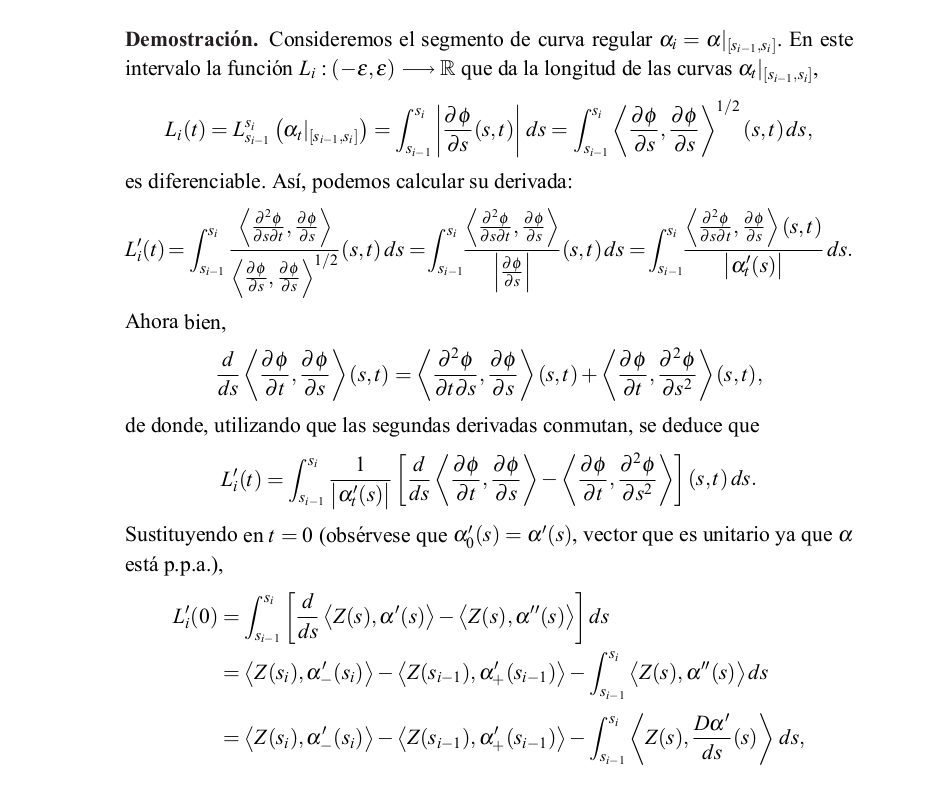
\includegraphics[width=\textwidth]{6.4i}
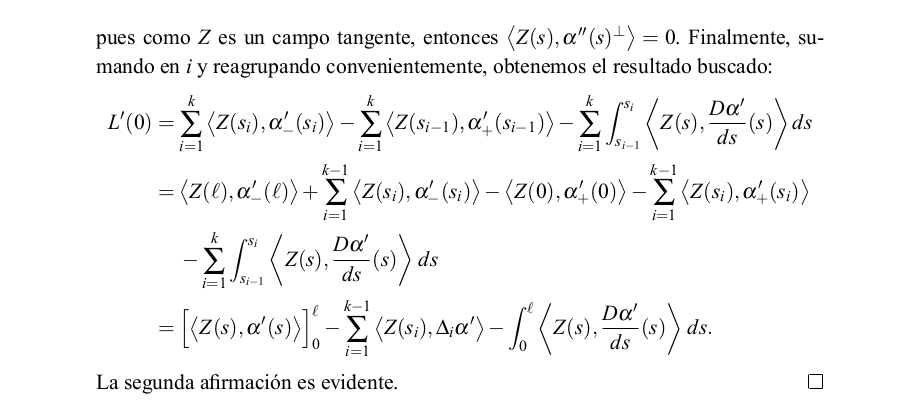
\includegraphics[width=\textwidth]{6.4ii}

\end{document}
